% TexStudio Spellchecking Command
% !TeX spellcheck = de_DE_OLDSPELL

%
% Copyright Clemens H. Cap (C) 2023
% Nutzung nach Creative Commons 4.0 BY-NC-SA
%

\documentclass[a4paper]{article}%   Könnte auch book sein, aber article setzt etwas kompakter und weniger Platz verschwendend

%%% Definiere aktuelle Dokumentenvariante
\def\mittext{}                 %% Für öffentliche Variante auskommentieren
%\def\instruktorflag{DEF}       %% Wenn definiert, dann sind auch Hinweise für Dozenten dabei. (Antworten, Namen von Referenzen)


\immediate\write18{path=('/opt/homebrew/bin/pygmentize' $path)}

\usepackage[multiple]{footmisc}

\def\missing{MISSING TODO!!!!!!!!!!!!!!!!!!!!!!!!!!!!!!!!!!!!!!!!!!!!!!!!!!!!!!!!!}

%%
%% common.tex  Macro Datei für den IW Reader
%%

\pdfoptionpdfminorversion=7                        % Anpassen PDF Version an die PDFs 
                                                   % die im reader eingebunden werden
%%
%% Import Packages
%%
\usepackage[german]{babel}                         % Sprache und Trenntabellen auswählen
\usepackage{geometry}                              % Anpassen Seitengeometrie für Einbau
                                                   % externer DPF-Dateien
                                                   
\usepackage{fontawesome}                           % Einige nette Symbole einbinden
\usepackage{dtk-logos}                             % Wir brauchen das Bibtex Logo
\usepackage{manfnt}                                % Benötigtes Symbol einbauen
\usepackage{MnSymbol,wasysym}                      % Benötigtes Symbol einbauen

\usepackage[inline]{enumitem}                      % Anpassbare Listen aktiv, inline
\usepackage{hhline}                                % Linien für farbige Tabellen
\usepackage[table]{xcolor}                         % Farbige Zellen in Tabellen
\usepackage{adjustbox}                             % Zusatz; rotierte Tabellen
\usepackage{tabto}                                 % Bessere Tabulatoren

\usepackage{fancyhdr}                              % Sinnvolle headings auf den Seiten
\pagestyle{fancy}                                  % Heading Stil aktivieren

\usepackage{qrcode}                                % QR Code setzen

\usepackage{pdfpages}                              % Importieren von PDF Dateien

\usepackage[outputdir=build,cache=false]{minted}   % Einbinden von Code mit Highlighting
                                                   % Option für build directory
                                                   % Caching aus wegen Selbstinklusion

\usepackage{graphics}                              % Grafiken einbauen
\usepackage{pgfplots}                              % Plot Funktionen
\usetikzlibrary{automata, positioning}             % Plot Libraries einbinden
\usetikzlibrary{arrows, arrows.meta}               % Plot Libraries einbinden

\usepackage{comment}                               % Teile auskommentieren
\usepackage{todonotes}                             % Notizen für den Autor

\usepackage{titletoc}                              % Partielle Inhaltsverzeichnisse

%%
%% Optik des Layout etwas nachjustieren
%%
\parindent 0pt                                     % Kein Paragrapheneinzug
\parskip   0.25cm                                  % Paragraphenabstand
\usepackage{titlesec}                              % \titlespaceing command
\titlespacing{\paragraph}{0pt}{8pt}{16pt}          % Paragraphen kompakter
\usepackage[all]{nowidow}                          % Hurenkinder, Schusterjungen vermeiden
\setlist[enumerate]{topsep=0pt}                    % Anpassbare Listen nutzen und anpassen
\setlist[itemize]{topsep=0pt}
\setlist[enumerate]*{label={(\arabic*)}}

%%
%% Neue Seite am Ende von \part vermeiden
%%
%
% Quelle: https://tex.stackexchange.com/questions/42526/
%         how-to-remove-page-break-after-part-in-report-book
%
\makeatletter
\def\@endpart{}                                   % First, modify the \@endpart macro.
\patchcmd{\part}{\null\vfil}{}{}{}                % Third, suppress vertical whitespace 
                                                  % before "Part xx" material
\makeatother

%%
%% Einstellungen für schönere Hyperlinks
%%
\usepackage{xurl}                                  % Erlaubt bessere Trennung von URLs
\usepackage[]{hyperref}                            % Hyperlinks  
                                                   % CAVE: load hyperref AFTER titlesec
\hypersetup{
  bookmarksnumbered=true,                          % number PDF
  breaklinks=true,                                 % may break links
  colorlinks,
  linkcolor={red},                                 % internal links 
  citecolor={red}, 
  urlcolor={blue},                                 % linked urls
  filecolor={blue}                                 % urls which open local files
}

\usepackage[type={CC},                             % Setup copyright notice
            modifier={by-nc-sa}, 
            version={4.0}]{doclicense}

%%
%% Einige Convenience Abkürzungen
%%
\def\PDF{\faFilePdfO PDF}
\def\online{\faExternalLink online}
\def\tikz{Ti\textit{k}Z}

%%
%% Macro, um die totale Seitenzahl des Readers zu ermitteln
%%
%
%  \pages{ <num> }    Addiert und gibt aus
%  \pages*{ <num> }   Addiert und gibt nicht aus
%  Zähler:            totalpages
%
\newcounter{totalpages}\setcounter{totalpages}{0}  % Lokalen Zähler anlegen
\makeatletter
\def\@pages#1{\addtocounter{totalpages}{#1}}%      % Makro Seitenzahl ohne Ausgabe
\def\@@pages#1{%
  \def\one{1}%
  \def\arg{#1}%
  (#1~\ifx\one\arg{Seite}\else{Seiten}\fi)%
  \addtocounter{totalpages}{#1}}%                  % Makro Seitenzahl MIT Ausgabe
\def\pages{\@ifstar\@pages\@@pages}%
\makeatother

%%
%% Referenzen über mehr als einen LaTeX-Lauf merken
%%
%
%  Bsp: Wert von totalpages am Ende des Dokuments in totalPageNumber speichern     
%       \storereference{totalPageNumber}{\thetotalpages}
%
%       Wert von totalPageNumber an anderer Stelle nutzen                    
%       \crtrefnumber{totalPageNumber}
%
\usepackage{crossreftools}
\crtrefundefinedtext{0}                            % Undefinierte Referenzen sind 0
\newcommand{\storeReference}[2]{\crtcrossreflabel*{#2}[#1]}


%%
%% \glabel definiert einen globalen label, der in \currentLabel gespeichert wird
%% Benötigt für die backlinks, wo eine Aufgabe etc benutzt wurde
%%
\def\glabel#1{\label{#1}\hypertarget{#1}{}\gdef\currentLabel{#1}}

%%
%% LATEXTRAINING
%%
%   \latexaufgabe  Setzt die Titel-Zeile für eine Aufgabe
%   \latexaufgabe{ <Bezeichnung-der-Aufgabe> }{ <label-zum-referenzieren-der-aufgabe> }
%
%   \uselatexaufgabe  Verweist auf eine Aufgabe im Text
%   \uselatexaufgabe{ <label-zum-referenzieren-der-aufgabe> }
%   Bsp: Wir bearbeiten \useaufgabe{ <label-zum-referenzieren-der-aufgabe> }
%
\def\latexaufgabe#1#2{%
  \stepcounter{latexaufgabencounter}%
  \subsection*{\phantomsection\relax \hypertarget{#2}{}#1%
     \ifdefined\instruktorflag{\hfill\color{gray}#2}\fi}%      
   \label{lt\thelatexaufgabencounter}%
  %   Referenznamen nur in Dozentenversion zeigen
  \addcontentsline{toc}{subsection}{#1}%
  \storeReference{#2}{#1}%    Speichere Bezeichnung unter dem label
}

\def\uselatexaufgabe#1{\hyperlink{#1}{\crtrefnumber{#1}}}

\newcounter{latexaufgabencounter}


%%
%% AUFGABEN
%%
%   \aufgabe  Setzt die Titel-Zeile für eine Aufgabe
%   \aufgabe{ <Bezeichnung-der-Aufgabe> }{ <label-zum-referenzieren-der-aufgabe> }
%
%   \useaufgabe  Verweist auf eine Aufgabe im Text
%   \useaufgabe{ <label-zum-referenzieren-der-aufgabe> }
%   Bsp: Wir bearbeiten \useaufgabe{ <label-zum-referenzieren-der-aufgabe> }
%
\def\aufgabe#1#2{%
  \stepcounter{aufgabencounter}%
  \hypertarget{#2}{}%        Target für \useaufgabe setzen
  \label{#2}% 
  \subsection*{\phantomsection\relax Aufgabe \theaufgabencounter:~#1%
     \ifdefined\instruktorflag{\hfill\color{gray}#2}\fi}%       
  % Referenznamen nur in Dozentenversion zeigen
  \addcontentsline{toc}{subsection}{Aufgabe \theaufgabencounter:~#1}%
  \storeReference{#2}{Aufgabe \theaufgabencounter:~#1}%     Speichere Mapping von 
                                         %  Aufgaben-Label zu Aufgabenbezeichnung
  \storeReference{AU#2}{\theaufgabencounter}%  Maps label to number
  \textbf{Behandelt:} In \nameref{\crtrefnumber{Label#2}}.
}
\def\useaufgabe#1{\hyperlink{#1}{\crtrefnumber{#1}}%
  \storeReference{Label#1}{\currentLabel}% Mapping von "Label" gefolgt 
  %         von Aufgaben-Label zu Label der Unit wo es behandelt wird
  \ifdefined\instruktorflag{\hfill\color{gray}#1} \fi%
}
\newcounter{aufgabencounter}

\def\sa#1{\hyperlink{#1}{\bf\crtrefnumber{AU#1}}}%  given a label provides a link to the aufgabe


%%
%% VORFÜHRUNGEN
%%
%
%  \demo  Setzt die 
%  \demo{ <Bezeichnung-der-Vorführung> }{ <label-zum-referenzieren-der-Vorführung> }
%  \usedemo{ <label-zum-referenzieren-der-Vorführung> }
%
\def\demo#1#2{
  \stepcounter{democounter}%
  \hypertarget{#2}{}%        Target für \usedemo setzen
  \subsection*{\phantomsection\relax Vorführung \thedemocounter:~#1%
    \ifdefined\instruktorflag{\hfill\color{gray}#2}\fi}%
  \label{vor\thedemocounter}%  vor<number> ist der label space der Vorführungen
  %  Referenznamen nur in Dozentenversion zeigen
  \addcontentsline{toc}{subsection}{Vorführung \thedemocounter:~#1}%
  \storeReference{#2}{Vorführung \thedemocounter:~#1}  
}
\def\usedemo#1{\hyperlink{#1}{\crtrefnumber{#1}}}
\newcounter{democounter}


%%
%% UNITS
%%
%   #1  Name to be written    
%   #2 Label used for referencing (needed in case of \LaTeX in title)
\newcounter{unitcounter}\setcounter{unitcounter}{0}%           Zähler für Units
\def\unit#1#2{%                                                Header für Leseeinheit setzen
  \clearpage%
  \stepcounter{unitcounter}%
  \setcounter{header}{1}%                                      Neue Nummerierung
  \lhead{Reader}%                                              Linke Header in Unit
  \rhead{Einheit \theunitcounter: #1}%                         Rechter Header in Unit
  \hypertarget{#2}{}%                                          Target setzen zur Unit
  \storeReference{#2}{Reader Einheit \theunitcounter:~#1}%
  \storeReference{Num#2}{\theunitcounter}%
  \section*{\phantomsection\relax Einheit \theunitcounter: #1%
    \ifdefined\instruktorflag{\hfill\color{gray}#2}\fi}%
    \label{unit\theunitcounter}%
  \addcontentsline{toc}{section}{Einheit \theunitcounter:~#1}%
  \gdef\unitName{#1}
}

\def\useunit#1{\hyperlink{#1}{\crtrefnumber{#1}}}% Referenziere ganze Reader Unit über Namen.

\def\uu#1{\hyperref[\crtrefnumber{#1}]{#1}}%  referenziere reader unit über namnen, zeige nummer

\newcounter{header}\setcounter{header}{1}%    Subzähler für einzelne Elemente in Einheiten

%%
%% Zur Formatierung jener Teile im Reader, die auf derselben Ebene wie die \units sind
%% die aber selber nicht Einheiten sind, und sich daher anders verhalten müssen (Links etc)
%% Bsp: Vorwort Nachwort
%%
\def\mysection#1{
  \clearpage%
  \lhead{Reader}%
  \rhead{#1}%
  \phantomsection%   \section* setzte keine hypertargets
  \section*{#1}%
  \addcontentsline{toc}{section}{#1}%
}

%%
%% Im Footer rechts überall einen Link zurück zum Inhaltsverzeichnis setzen
%%
\rfoot{\hyperlink{Inhaltsverzeichnis}{\faListOl}}% 

%%
%% Pagestlye für den Reader / PDF Import setzen
%%
%  Quelle in den Footer schreiben.
%
\fancypagestyle{pdfpages}{%                       Page style für Reader definieren
  \renewcommand{\headrulewidth}{0pt}%             Keine Trennlinie im Header, denn wir haben 
%                                                 einen Rahmen in variabler Länge je nach
%                                                 Größe der importierten Seite
  \fancyfoot[L]{\footnotesize\pdfpagesfooter}
  \fancyfoot[C]{}%                                Zentrierter Footer wäre die Seitenzahl, 
  %                                               die wir im Reader nicht brauchen
  \fancyfoot[R]{\hyperlink{Inhaltsverzeichnis}{\faListOl}\hspace*{-1cm}}%
}

\newcommand*\pdfpagesfooter{}

\newcommand{\setlayout}[1]{%               Macro um Page Style (footer) auf der 
%                                          spezifischen Seite des PDF Include zu setzen
  \thispagestyle{pdfpages}%                Auf pdfpages page style umschalten
  \gdef\pdfpagesfooter{#1}%                Parameter in globaler Variablen speichern
}


%%
%% Pagestyle für den Anhang definieren
%%
\fancypagestyle{anhang}{
  \fancyhead[L]{}
  \fancyhead[C]{Anhang}%                                
  \fancyhead[R]{}%
}





%%
%% READER-INHALT
%%
%
%  \add         Definieren ein Inhaltselement im Reader
%    #1 Header Text für den Inhalt, dient auch als Label für Verweise    
%       CAVE:   Darf keine Sonderzeichen enthalten wegen Nutzung als Label
%    #2 Text der den Inhalt beschreibt
%    #3 Filename des Inhalts, inklusive Pfad                    oder leer {}
%    #4 Ein vollständiger Link is web in der Form \href{}{}     oder leer {}
%
\makeatletter
\newwrite\appendFile
\immediate\openout\appendFile=appendFiles.lst
\def\add#1#2#3#4{%
  \hypertarget{Kom:#1}{}%                        Target für das Kommentar setzen
  \textbf{\S \theunitcounter.\theheader:~#1} #2%  
  \def\argFile{#3}%                              Parameter in Variable speichern 
  %                                              nötig für Vergleich mit leerem Macro
  \ifx\argFile\empty\else%                       Wenn File vorhanden, 
    \relax\space\hyperlink{Ank:#1}{\PDF}\fi%     Link setzen auf Ankündigungsseite
  \def\argu{#4}%
  \ifx\argu\empty\else\relax\space\argu\fi%
  \ifx\argFile\empty\else%                       Wenn File vorhanden, 
    \write\appendFile{%                          Ankündigungsseite;  File inkludieren
      \unexpanded{\hypertarget}{#3}{}%
      \unexpanded{\hypertarget}{Ank:#1}{}%       Target für die Ankündigungsseite
      \unexpanded{\rhead{}\lhead{}}%             Header der Ankündigungsseite löschen
      \unexpanded{\chead}{\footnotesize\textbf{Einheit \theunitcounter:~\unitName}% 
        \hfill \textbf{Text:}~#1}%               Header Ankündigungsseite  
      \unexpanded{\phantomsection}%
      \unexpanded{\addcontentsline}{toc}{section}{#1}%
      \unexpanded{\large}%
      \unexpanded{\renewcommand\baselinestretch{1.2}}%
      \unexpanded{\topskip0pt\vspace*{\fill}}%
      \unexpanded{\textbf}%
      {#1} \\[6pt]%
      #2   \\[6pt]%
      #4
      \unexpanded{\vspace*{\fill}}%
      \unexpanded{\normalsize}%
      \ifdefined\mittext
        \unexpanded{\includepdf[pages=-, 
                                pagecommand=\setlayout{\textbf{Quelle:}~#2}, 
                                width=\textwidth,
                                height=\textheight,
                                keepaspectratio,
                                frame]}{#3}%
      \else\par
         Den Text finden Sie aus urheberrechtlichen Gründen nur 
         in der eingeschränkten Variante dieses Dokuments oder
         online unter der Verantwortung der entsprechend verlinkten Site.
         \vfill\pagebreak
      \fi
     %
      }%
  \fi%
  \stepcounter{header}%
}
\makeatother

\usepackage{csquotes}                         % Quotes; Paket möglichst spät laden

\ifdefined\instruktorflag%                      Wenn instruktorflag gesetzt
  \usepackage[firstpageonly=true]{draftwatermark}% Watermark auf Frontseite zur Warnung
\fi
%                %% Style File für den Reader einlesen

\title{Informatik, Wissenschaft, Gesellschaft \\[12pt] \normalsize Arbeitsmaterialien, Aufgabensammlung und Reader}
\author{Clemens H. Cap}
\date{\today, Version 1.1}

\begin{document}

\maketitle

\ifdefined\instruktorflag\SetWatermarkText{Interne Version}\SetWatermarkScale{3}\fi

\begin{quote}

\textbf{Hinweis:} Aus urheberrechtlichen Gründen gibt es dieses Dokument in zwei Varianten.
Die \textit{öffentliche Variante} enthält nur die Referenzen auf die Texte des Readers.
Die \textit{eingeschränkte Variante} wendet sich an die Teilnehmer meiner entsprechenden Lehrveranstaltung
und gibt im Teil 3 (Reader) auch die zitierten Texte wieder.
Die Wiedergabe richtet sich dabei nach \href{https://dejure.org/gesetze/UrhG/60a.html}{\S 60a UrhG}, 
weshalb sie nur hochschulintern zugänglich ist.

\ifdefined\mittext\textbf{Dieses Exemplar ist die eingeschränkte Variante.
Sie darf daher weder weitergegeben noch uneingeschränkt öffentlich
zugänglich gemacht werden.}
\else\textbf{Dieses Exemplar ist die öffentliche Variante.}\fi

\vfill

\textbf{Copyright in den Teilen 1 und 2:}  Clemens H. Cap, \copyright 2024.
\doclicenseThis

\textbf{Copyright im Teil 3:} Es gilt das Copyright der jeweiligen Rechteinhaber.

\vfill

%\begin{tabular}[]{@{}c@{}}  % Doppelte @{} um komplett bündig zu setzen
%\qrcode[hyperlink,height=2in]{https://iuk.one} \\  \\[2pt] 
%\href{https://iuk.one}{Verteilung auf https://iuk.one}
%\end{tabular}\hfill\begin{tabular}[]{@{}c@{}}
%\qrcode[hyperlink,height=2in]{https://github.com/clecap/vorlesung-informatik-und-wissenschaft/settings} 
%\\ \\[2pt]
%\href{https://github.com/clecap/vorlesung-informatik-und-wissenschaft}{Quellen des Dokuments} \\
%\href{https://github.com/clecap/vorlesung-informatik-und-wissenschaft}{auf https://github.com/clecap/}
%\end{tabular}

%\vfill

%Hinweise auf Fehler im Dokument bitte im Repository 
%\url{https://github.com/clecap/vorlesung-informatik-und-wissenschaft}
%als \href{https://github.com/clecap/vorlesung-informatik-und-wissenschaft/issues}{\textit{issue}} %einpflegen.

\end{quote}

\clearpage

\subsection*{Versionsgeschichte}


\textbf{Version 1.1}

Die vorliegende Version ist eine vorläufige Version, bei der noch etliche Teile ergänzt werden, da Teile der Lehrveranstaltung
parallel zum laufenden Semester vorbereitet werden.

% TODO: Quellen auf Github einstellen.

% TODO: QR Code Links prüfen

\clearpage

\vspace*{\fill}

{\raggedright
\begin{quote}
Alle Hindernisse und Schwierigkeiten sind Stufen,\\
auf denen wir in die Höhe steigen.\\[12pt]
\hfill \textsc{Friedrich Nietzsche}\footnote{\textsc{Nietzsche} zugeschrieben nach: H. Brosche: Warum es nicht so schlimm ist, in der Schule
schlecht zu sein. Kösel-Verlag, 2009. Siehe aber auch: \url{https://falschzitate.blogspot.com/2019/05/hindernisse-und-schwierigkeiten-sind.html}.}, Deutscher Philosoph
\end{quote}
}


{\raggedright
\begin{quote}
Bildung ist letztlich viel mehr \\ als einzelne Fakten auswendig zu lernen.\\
Was am wichtigsten ist: \\ Lernen selber zu denken, \\ lernen zu argumentieren und \\ lernen wie man am besten lernt.\footnote{Quelle: \url{https://de.wikipedia.org/wiki/Vitalik\_Buterin}.}\\[12pt]
\hfill\textsc{Vitalik Buterin}, Mitbegründer von Ethereum
\end{quote}
}

\clearpage


\clearpage

\pagebreak\hypertarget{Inhaltsverzeichnis}{}
\tableofcontents


\clearpage


\part{Übersicht und Aufgabensammlung}

\startcontents[part1]
\printcontents[part1]{}{1}[1]{}

\clearpage%  Force start on next page and thereby improve positioning of PDF bookmark target; due to my use of article style


\section{Ziel und Inhalte}\label{ZieleUndInhalte}

\paragraph{Ziel:} Die Lehrveranstaltung \enquote{Informatik, Wissenschaft, Gesellschaft} (IWG) 
behandelt die Grundlagen des wissenschaftlichen Arbeitens in Informatik und beleuchtet
die Spannungsfelder zwischen Informatik und Gesellschaft sowie zwischen
Wissenschaft und Gesellschaft.

Die Veranstaltung knüpft damit an die Lehrveranstaltung \enquote{Informatik und Wissenschaft} (IW)
an, die im 2. Semester des Bachelor-Studiums eine erste Einführung in
wissenschaftliches Arbeiten in Informatik gegeben hat.

Standen in der IW die praktischen Fertigkeiten wissenschaftlichen Arbeitens
im Vordergrund, so konzentriert sich die IWG
stärker auf die systematischen und theoretischen Hintergründe von Wissenschaft. Sie beleuchtet
ferner das Spannungsfeld zwischen Informatik und Gesellschaft und baut dabei auf die
im Fachstudium Informatik erworbenen Kenntnisse jener Themen auf, die gesellschaftliche 
Problemfelder von Technik und Wissenschaft betreffen.


\paragraph{Inhalte:} In der Veranstaltung IW wurden die folgenden Themenfelder behandelt:
\begin{enumerate}
\item \textbf{Lernen:} \hfill Strategien für ein leichteres und effizienteres Lernen.
\item \textbf{Wissenschaft:} \hfill Einführung in wissenschaftliches Arbeiten und Methoden.
\item \textbf{Organisieren:} \hfill Zeit- und Selbstmanagement, Strategien zum Meistern des Studiums.
\item \textbf{Lesen:} \hfill Techniken des schnellen und des auswertenden Lesens.
\item \textbf{Literatur:} \hfill Arbeiten mit wissenschaftlicher Literatur.
\item \textbf{Schreiben:} \hfill Wissenschaftlicher Schreibstil.
\item \textbf{Vortragen:} \hfill Gestaltung eines Vortrags.
\item \textbf{Paper:} \hfill Praktische Übung anhand eines kurzen Papiers.
\item \textbf{\LaTeX:} \hfill Einführung in den Textsatz für Ingenieur- und Naturwissenschaften.
\end{enumerate}

\bigskip


\paragraph{Inhalte:} In der Veranstaltung IWG werden nun die folgenden Themenfelder behandelt:
\begin{enumerate}
\item \textbf{Wiederholung:} \hfill Wiederholung der Inhalte der Grundlagenvorlesung IW.
\item \textbf{Wissenschaft:} \hfill Wissenschaftliches Arbeiten und Einführung in Wissenschaftstheorie.
\item \textbf{Bachelorarbeit:} \hfill Erstellen längerer wissenschaftlicher Arbeiten (Bachelor-Arbeit)
\item \textbf{Gesellschaft:}  \hfill Gesellschaftliche Themen der Informatik
\end{enumerate}


Wegen ihrer hohen Bedeutung werden die folgenden Themenfelder aus der IW im Rahmen 
der IWG, speziell in den Übungen, nochmals wiederholt und gefestigt:









\clearpage


\clearpage
\section{Organisation und Ablauf}\label{OrganisationUndAblauf}

\subsection{Elemente}

Die Lehrveranstaltung umfaßt die folgenden Elemente:

Die \hyperref[Digitalvorlesung]{\textbf{Digitalvorlesung}} besteht aus aufgenommenen Vorlesungen (Video/Audio-Strom sowie
Unterlagen in PDF-Form). Sie dient der ersten Wissensvermittlung.
Sie wird von Ihnen \textit{nach eigenem Zeitplan selb\-ständig} angesehen und individuell oder in selbstorganisierten Gruppen erarbeitet.
Die dabei entstandenen Fragen bringen Sie in die Präsenzvorlesung mit.

Die \hyperref[Prsenzvorlesung]{\textbf{Präsenzvorlesung}} arbeitet nach dem Modell des \textit{inverted} oder 
\textit{flipped classroom}\footnote{Mehr dazu siehe \url{https://www.e-teaching.org/lehrszenarien/vorlesung/inverted_classroom}.}
Dieses setzt eine Beschäftigung mit den Materialien
der Digitalvorlesung und des Readers (s. unten)
als Vorbereitung  voraus. 
Die Veranstaltung wiederholt und diskutiert das erworbene Wissen.
Dabei können entstandene Fragen geklärt werden.
In der gemeinsamen Anwendung des Wissens auf Beispiele
sollen Grenzfälle ausgelotet werden und die eigene Modellbildung kann auf
den Prüfstand gestellt werden.
Da der Stofferwerb teilweise bereits vor der Präsenzvorlesung erfolgt ist, kann dabei eine
Kontrolle und ein Nachjustieren der erworbenen Kenntnisse erfolgen.

Die \hyperref[Ubung]{\textbf{Übung}} setzt eine \textit{vorangehende Bearbeitung} von Übungsaufgaben voraus.
Sie dient der praktischen Einübung von Standardverfahren des wissenschaftlichen Arbeitens; sie bietet
Raum für weitere Diskussionen und ergänzende Sichtweisen.

Die \hyperref[auf]{\textbf{Aufgaben}} umfassen Fragestellungen, die zu einer intensiveren praktischen
Beschäftigung mit dem Stoff anregen. Jede Aufgabe
wird entweder in einer Präsenzvorlesung oder in einer Übung mit den Teilnehmern behandelt.

Besondere Bedeutung kommt den Aufgaben bei der Behandlung gesellschaftlicher und ethischer Fragen zu,
da die Antworten auf diese Fragen gesellschaftlich gerade im Entstehen begriffen sind.
Es gibt oftmals keine \enquote{richtigen} Antworten, da diese von den persönlichen
Wertesystemen abhängen und diese wieder alters-, kultur- und generationsspezifische Perspektiven
und Erfahrungen voraussetzen; zudem ist hier auch das einzelne Individuum gefragt!
Hier kommt der persönlichen Mitarbeit eine besondere Bedeutung zu. In der Prüfung werden die gemeinsam erarbeiteten
Überlegungen ebenso von Bedeutung sein. Daher wird eine aktive Teilnahme an den Diskursen in 
Übung und Präsenzvorlesung besonders empfohlen.

Der \hyperref[Reader1]{\textbf{Reader}} besteht aus einer kommentierten Auswahl von Texten. Er dient der Ergänzung der
Digitalvorlesung. Er soll zu einer weitergehenden Befassung mit dem Stoff anregen und Ausgangspunkt für
Fragen und Diskussionen in der Präsenzvorlesung und in der Übung sein.
Einzelne Elemente der Lehrveranstaltung verweisen daher auf Teile des Readers.






\pagebreak



\subsection{Struktur}

\todo{TBD=To Be Defined}

% Definition von Farbzellen
\def\blu{\cellcolor{blue!25}}
\def\red{\cellcolor{red!25}}
\def\yel{\cellcolor{yellow!25}}
\def\gre{\cellcolor{green!25}}


\def\VL#1{\hyperref[VLIW#1]{\textbf{VL #1}}}
\def\UE#1{\hyperref[UEIW#1]{\textbf{UE #1}}}

\def\H#1{\hyperref[H#1]{\textbf{#1}}}

\def\V#1{\hyperref[vor#1]{\textbf{#1}}}

\def\LT#1{\hyperref[lt#1]{\textbf{#1}}}
\def\U#1{\hyperref[unit#1]{\textbf{#1}}}



%%
%% CONFIGURE
%%
% vorlesung time
\def\vlt{13.00-14:30}

\def\uee{11:00-12:30}
\def\uez{11:00-12:30}







% https://tex.stackexchange.com/questions/32683/rotated-column-titles-in-tabular
% Schiefen Tabellenheader setzen
\newcolumntype{R}[2]{%
  >{\adjustbox{angle=#1,lap=\width-(#2)}\bgroup}%
  l%
  <{\egroup}%
}
\newcommand*\rot{\multicolumn{1}{R{45}{1em}}}% no optional argument here, please!




{\setlength{\arrayrulewidth}{1.0pt}% Helps to prevent line color from being overwritten by cell color 
\setlength\extrarowheight{4pt}
\begin{table}[h]
\begin{center}
\begin{tabular}[]{@{}|l|c|c|c|c|c|c|c|c|c|c|c|}
 \multicolumn{1}{c}{} &\rot{\bf \hyperref[latex]{Literatur (WH)}} &  \rot{\bf \hyperref[vor]{Gliederung \& Aufbau}} & \rot{\bf \hyperref[Hausarbeit]{Schreiben}} & \rot{\bf Bachelorarbeit}  & \rot{\bf TBD}&\rot{\bf TBD}& \rot{\bf TBD} &\rot{\bf TBD}& \rot{\bf TBD} & \rot{\bf TBD} & \rot{\bf TBD}   \\[1pt] \hline
\multicolumn{12}{c}{\bf\large Vorlesungen} \\ \hline
\VL1 & \blu  & \blu  & \blu &  &           &                      &                    &                      &              &       &  \\
\VL2 &  &  &&      &                       &                 &                    &                     &              &       &     \\
\VL3 &  &  &&      &                       &                      &                    &                     &              &      &    \\
\VL4 &  &  &&      &                  &                      &                    &                    &           &      &     \\
\VL5 &  &  &&      &                  &                      &                    &                        &          &      &   \\
\VL6 &  &  &  &      &                  &                      &                    &                        &              &   & \\ \hline 
\multicolumn{12}{c}{\bf\large Übungen} \\ \hline
\UE1 & \blu   &     &            &  &                  &                      &                    &                      &              &       &  \\
\UE2 &   & \blu     &    &  &                       &                 &                    &              &              &       &     \\
\UE3 &    &      &  \blu          &  &                       &                      &              &            &              &       &   \\
\UE4 &    &            &              &  &                       &                      &                    &                       &            &       &    \\
\UE5 &    &            &      &  &                       &                      &                    &                        &        &        &  \\
\UE6 &    &            &     &  &                   &                      &                    &                        &              &   &  \\ 
\UE7 &    &            &      &  &                  &                      &                    &                        &              &   &  \\ \hline
\end{tabular}
\end{center}
\caption[Struktur der Übungen]{\textbf{Übersicht über die Struktur} der Vorlesungen und Übungen: In welchen Stunden behandeln wir welche Themenfelder?}
\label{tab:uebungsstoff}
\end{table}
}


\clearpage

\subsection{Was ist vorzubereiten?}

\todo{Ergänzungen folgen}

Die einzelnen Elemente der Lehrveranstaltung sind miteinander verzahnt.
Damit leichter ersichtlich wird, auf wann was vorbereitet werden soll, habe ich
die folgenden beiden Tabellen erstellt:


{\setlength{\arrayrulewidth}{1.0pt}% Helps to prevent line color from being overwritten by cell color 
\begin{table}[h]
\begin{center}
\begin{tabular}[]{@{}l|c|c|c|c|c|c|c|}
                                & \rot{\bf \hyperref[auf]{Aufgaben}} &  \rot{\bf \hyperref[Reader1]{Reader}} &\rot{\bf \hyperref[DV]{DigitalVL}} \\[1pt] \hline
\VL1 &                & \yel  \U1, \U2&   \gre \hyperref[DV]{\bf DV1}, \hyperref[DV]{\bf DV3}, \hyperref[DV]{\bf DV7}     \\
\VL2 &                &  &      \\
\VL3 &                &  &       \\
\VL4 &                &   &        \\
\VL5 &                &   &      \\
\VL6 &                 &     &   \\ \hline
\end{tabular}
\end{center}
\caption[Vorbereitung auf die Präsenzvorlesungen]{\textbf{Vorbereitung auf die Präsenzvorlesungen:} Bis wann ist was vorzubereiten? 
Welche Aufgaben sind vorzubereiten?
Welche Einheiten im Reader sollen bis wann gelesen werden? 
Welche Digitalvorlesungen sollen wann angesehen werden?
Bei \VL1 handelt es sich um eine \textit{Nach}bereitung, in allen anderen Fällen um eine \textit{Vor}bereitung.
}
\label{tab:preparevl}
\end{table}
}





%\item \useaufgabe{GliederungenErstellen}
%\item \useaufgabe{ForschungsfrageChat}
%\item \useaufgabe{WunschthemaFormulieren}



{\setlength{\arrayrulewidth}{1.0pt}% Helps to prevent line color from being overwritten by cell color 
\begin{table}[h]
\begin{center}
\begin{tabular}[]{@{}l|c|c|c|c|c|c|}
                                 &  \rot{\bf \hyperref[auf]{Aufgaben}} & \rot{\bf \hyperref[Reader1]{Reader}} &\rot{\bf \hyperref[DV]{DigitalVL}} \\[1pt] \hline
\hyperref[UEIW1]{\textbf{UE 1}}  &                              &  &     \gre \hyperref[DV]{\bf DV1}   \\
\hyperref[UEIW2]{\textbf{UE 2}}  &   \sa{GliederungenErstellen},\sa{ForschungsfrageChat}, \sa{WunschthemaFormulieren}   & \yel \U1  &  \gre \hyperref[DV]{\bf DV7}      \\
\hyperref[UEIW3]{\textbf{UE 3}}  &                 &   &       \\
\hyperref[UEIW4]{\textbf{UE 4}}  &                 &   &        \\
\hyperref[UEIW5]{\textbf{UE 5}}  &                 &   &            \\
\hyperref[UEIW6]{\textbf{UE 6}}  &                 &    &   \\ 
\hyperref[UEIW6]{\textbf{UE 7}}  &                 &    &   \\ 
\hline
\end{tabular}
\end{center}
\caption[Vorbereitung auf die Übungen]{\textbf{Vorbereitung auf die Übungen:}
Welche \LaTeX-Trainings sind vorzubereiten?
Welche Aufgaben sind vorzubereiten?
Wann finden welche Vorführungen statt?
Wann sprechen wir über die Hausarbeit?
Welche Einheiten im Reader sollen bis wann gelesen werden? Welche Digitalvorlesungen sollen wann angesehen werden?}
\label{tab:prepare}
\end{table}
}


\clearpage


\subsection{Arbeitsaufwand des Moduls}

\begin{table}[h]\label{arbeitsaufwand}
\begin{center}
\begin{tabular}[]{@{}|l|r|}
\hline
  \multicolumn{1}{|c}{\hspace*{2cm}\textbf{Aktivität}\hspace*{2cm}}         & 
  \multicolumn{1}{c|}{\textbf{Zeitbedarf}} 
 \rule{0pt}{4ex} \\[4pt]\hline
\rule{0pt}{3ex}%
\hspace*{1cm}{\em Präsenzvorlesung}                  & $6\times 2 = 12$ Std   \\
\hspace*{1cm}{\em Übung}                             & $7\times 2 = 14$ Std   \\
\multicolumn{1}{|l|}{Summe Anwesenheiten}                    & $26$ Std               \\
\hspace*{1cm}{\em Digitalvorlesung}                  &  $5 + 7 = 12$ Std\footnotemark               \\
\hspace*{1cm}{\em Reader}                            &  $22$ Std              \\
\multicolumn{1}{|l|}{Summe strukturiertes Selbststudium}   & $34$ Std   \\
\multicolumn{1}{|l|}{Vorbereitungszeit für die Aufgaben}             & $15$ Std   \\
\multicolumn{1}{|l|}{Prüfungsvorbereitung}   & 15 Std                             \\[4pt]\hline
\multicolumn{1}{|c|}{\textbf{Total}}                 &  \textbf{90 Std} \rule{0pt}{4ex}    \\[4pt]\hline
\end{tabular}
\end{center}
\caption[Zeitbilanz der Veranstaltung]{Zeitbilanz der Veranstaltung: 3 Leistungspunkte = 90 Stunden Zeitaufwand.}

\end{table}


\footnotetext[4]{Ergeben sich aus den Zeiten der Digitalvorlesungen der IWG (5) und den Zeiten 
der Digitalvorlesungen der IW (7), die \textbf{beide} zum Stoff- und Prüfungsumfang in der IWG gehören.}


\clearpage




\subsection{Ablauf}




\subsubsection{Präsenzvorlesung}

\textbf{Zeit:} Die Veranstaltung ist auf 6 Präsenzvorlesungen im Semester ausgelegt.
Die Zeitplanung richtet sich nach Tabelle \ref{tab:vlzeit}. 

\textbf{Ort:} Die Veranstaltung findet in der Albert-Einstein-Strasse 22 (Zusehaus) in Raum 037 statt.

\begin{table}[h]
\begin{center}
\begin{tabular}[]{@{}|lll|}\hline\rule{0pt}{2.5ex}%
\VL1 & Fr 25. 10. 2024. & \vlt \\ 
\VL2 & Fr 08. 11. 2024. & \vlt \\
\VL3 & Fr 06.  12. 2024. & \vlt \\
\VL4 & Fr 20. 12. 2024. & \vlt \\
\VL5 & Fr 17. 01. 2025. & \vlt \\
\VL6 & Fr 31. 01. 2025. & \vlt \\\hline
\end{tabular}
\end{center}
\caption{Zeitplan der Präsenzvorlesung.}
\label{tab:vlzeit}
\end{table}

\subsubsection{Übung}

\textbf{Zeit:} Die Veranstaltung ist auf 7 Übungstermine im Semester ausgelegt. Davon ist die
1. Übung eine Wiederholung zur Lehrveranstaltung IW.

\textbf{Ort:} Die Veranstaltung findet in der Albert-Einstein-Strasse 22 (Zusehaus) 
in Raum SR 101 statt.

\begin{table}[h]
\begin{center}
\begin{tabular}[]{@{}|c|lr|lr|lr|}\hline
    \rule{0pt}{4ex}
     &  \multicolumn{2}{c|}{\textbf{Gruppe 1}}  
     &  \multicolumn{2}{c|}{\textbf{Gruppe 2}}      
          \\[6pt]\hline\rule{0pt}{3ex}%
\UE1 &   Mi  23. 10. 2024 & \uee   & Mi 16. 10. 2024   & \uez     \\
\UE2 &   Mi  06. 11. 2024 & \uee   & Mi 30. 10. 2024   & \uez    \\
\UE3 &   Mi  20. 11. 2024 & \uee   & Mi 13. 11. 2024   & \uez    \\
\UE4 &   Mi  04. 12. 2024 & \uee   & Mi 27. 11. 2024   & \uez     \\
\UE5 &   Mi  18. 12. 2024 & \uee   & Mi  11. 12. 2024  & \uez    \\
\UE6 &   Mi  15. 01. 2025 & \uee   & Mi  08. 01. 2025  & \uez     \\
\UE7 &   Mi  29. 01. 2025 & \uee   & Mi  22. 01. 2025  & \uez     \\
\hline

\end{tabular}
\end{center}
\caption{Zeitplan der Übung.}
\label{tab:uebungszeit}
\end{table}

\pagebreak

\subsubsection{Übersicht}

Für die einzelnen Übungsgruppen ergeben sich daraus die Präsenzveranstaltungen aus Tabelle~\ref{tab:insgesamt}.

\begin{table}[h]
\begin{center}
{\setlength{\arrayrulewidth}{1.1pt}% Helps to prevent line color from being overwritten by cell color 
\setlength\extrarowheight{4pt}
\begin{tabular}[]{@{}|c|c|c|} \hhline{-|-|-}
        &  {\yel \textbf{Gruppe 1}}  & \multicolumn{1}{c|}{\yel \textbf{Gruppe 2}}   \\ \hline
16. 10. 2024 &         & \gre \UE1 \uez                                              \\ \hline
23. 10. 2024 &  \gre \UE1 \uee        &                                                \\ \hline
25. 10. 2024 &  \blu \VL1 \vlt   & \blu \VL1  \vlt       \\ \hline
30. 10. 2024 &         & \gre \UE2 \uez                                              \\ \hline
06. 11. 2024 &  \gre \UE2 \uee        &                                                \\ \hline
08. 11. 2024 &  \blu \VL2 \vlt   & \blu \VL2 \vlt     \\ \hline
13. 11. 2024 &         & \gre \UE3 \uez                                              \\ \hline
20. 11. 2024. &  \gre \UE3 \uee        &                                                \\ \hline
06. 12. 2024  &  \blu \VL3 \vlt   & \blu \VL3 \vlt     \\ \hline
27. 11. 2024 &         & \gre \UE4 \uez                                              \\ \hline
04. 12. 2024 &  \gre \UE4 \uee        &                                                \\ \hline
20. 12. 2024  &  \blu \VL4 \vlt   & \blu \VL4 \vlt    \\ \hline
11. 12. 2024 &         & \gre \UE5 \uez                                              \\ \hline
18. 12. 2024 &  \gre \UE5 \uee        &                                                \\ \hline
17. 01. 2025 &  \blu \VL5 \vlt   & \blu \VL5 \vlt   \\ \hline
08. 01. 2025 &         & \gre \UE6 \uez                                              \\ \hline
15. 01. 2025 &  \gre \UE6 \uee        &                                                \\ \hline
22. 01. 2025 &         & \gre \UE7 \uez                                              \\ \hline
29. 01. 2025 &  \gre \UE7 \uee        &                                                \\ \hline
31. 01. 2025 &  \blu \VL6 \vlt  & \blu \VL6 \vlt       \\ \hline
\end{tabular}
}
\end{center}
\caption{Gesamtansicht der Zeitplanung.}
\label{tab:insgesamt}
\end{table}




%\begin{figure}
%\begin{center}
%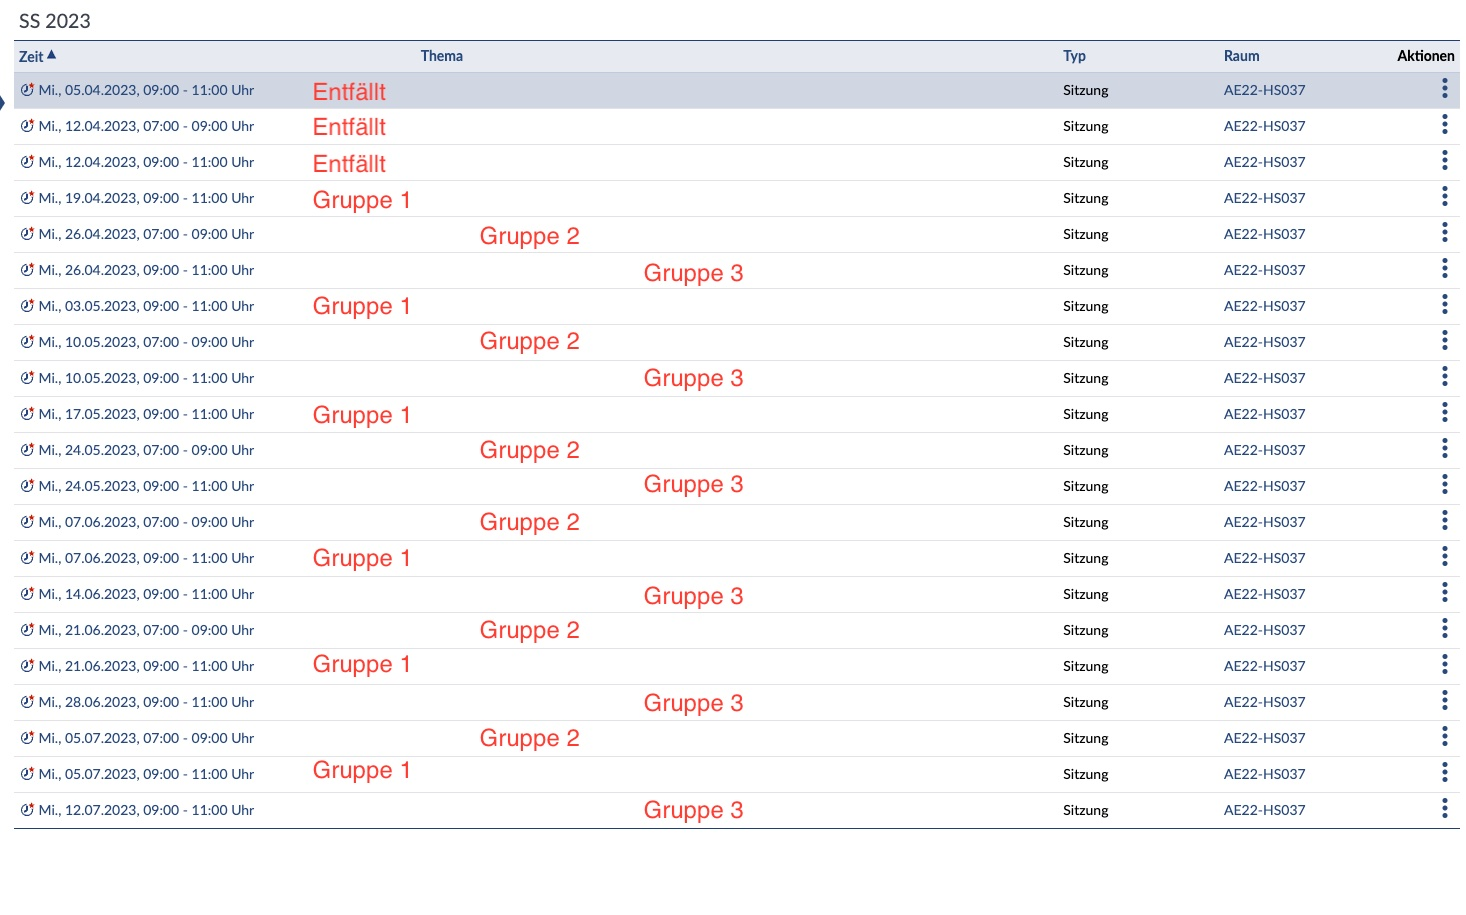
\includegraphics[scale=0.35,angle=90,origin=c]{zeitplan-studip-2023.jpg}
%\end{center}
%\caption{Abgleich mit der Planung auf StudIP.}
%\end{figure}


\clearpage



\section{Didaktische Überlegungen}

Der Stil dieses Textes ist \textit{nicht} der Stil, den Sie für die eigene wissenschaftli\-che
Arbeit nutzen sollten. In einer wissenschaftlichen Arbeit ist der \textit{intersubjektive Schreibstil}
wichtig, 
während hier ein anderes, nämlich ein \textit{didaktisches und motivationelles} Ziel im Vordergrund steht.
Gleichwohl kann der Reader als Beispiel dienen, wie Texte gegliedert und satztechnisch
aufbereitet werden können.

Die Anforderungen an den
wissenschaftlichen Schreibstil werden wir im Laufe dieses Kurses besprechen.
Trotzdem wollen wir hier zur Abgrenzung einige Unterschiede nochmals besonders herausarbeiten:

\paragraph{Schreibstil:}
Mit meinem Stil hier versuche ich, Sie zu motivieren, Sie durch den Lesevorgang zu begleiten und die
Lektüre kurzweilig zu gestalten. Daher schreibe ich im persönlichen \textit{ich}-Stil,
nutze rhetorische Fragen, erzeuge gelegentlich einmal Widersprüche, bevor ich diese wieder auflöse usw.
Das soll den Text spannend machen und zum Nachdenken anregen.
In einer wissenschaftlichen Arbeit ist das nicht immer angebracht -- ausgenommen Sie verfolgen dort,
beispielsweise in der Einleitung oder in der Zusammenfassung ein ähnliches Ziel.

\paragraph{Layout:} Mit meinem Layout versuche ich, die Struktur und die Zusammenhänge
zwischen den einzelnen Lehrelementen herauszuarbeiten. Der Text soll dadurch leichter lesbar
werden. Sicher ist das auch ein sinnvolles Ziel für eine Belegarbeit. Andererseits sollte
eine Belegarbeit auch eine gewisse minimale Länger haben -- was einem Layout mit viel \enquote{Luft}
zuwiderläuft.

\paragraph{Fußnoten:}
Für die Informatik ungewöhnlich ist die intensive Nutzung von Fußnoten. Diese werden hier
gebraucht, um Kontexte zu Aussagen zu setzen, Dinge zu hinterfragen, nach einer 
überspitzten Formulierung wieder zurecht zu rücken, sowie um Zusatzinformationen zu geben.

In geisteswissenschaftlichen Arbeiten finden sich häufig sehr viele Fußnoten,
in den Ingenieur- und Naturwissenschaften stellen sie eher eher die Ausnahme dar.
Es handelt sich hier um eine Tradition der jeweiligen Disziplinen.
Zudem: In Wissenschaften, die überzeugt davon sind, die Dinge durch Definitionen formal präzise 
beschrieben zu können entsteht seltener der
Bedarf, zu kontextualisieren oder zurecht zu rücken.

\paragraph{Zitate:}
Dieser Reader arbeitet mit Hypertext-Links, die in PDF durch \LaTeX\ erzeugt werden. 
Wenn Sie ihn in einem Standard-kompatiblen
PDF-Reader betrachten, so können Sie direkt den farbigen Links folgen.

Diese Art der Einbindung von Zitaten orientiert sich an der digitalen Welt, ist auf
Webseiten und Blogs üblich und erlaubt einen raschen Zugriff auf die zitierte Stelle.
Aus wissenschaftlicher Sicht wäre das aus etlichen Gründen problematisch: Das Link-Ziel ist
einer auf Papier gedruckten Version des Readers nicht immer zu entnehmen\footnote{Der Reader behebt dieses 
Problem teilweise,
indem er -- meistens -- auch ein vollständiges Literaturzitat angibt. Diese Vorgehensweise ist
in einer wissenschaftlichen Arbeit jedenfalls erforderlich.}; 
ein Link ist manchmal sehr lang oder enthält viele Sonderzeichen und ist damit 
nicht gut für den menschlichen Gebrauch
oder den Abdruck in einem Dokument geeignet\footnote{In diesem Fall würde man in einer gedruckten
Arbeit den Link eher nicht einarbeiten, vorausgesetzt, das Literaturzitat ist durch die anderen Angaben
hinreichend präzise angegeben.}; Links bieten keine stabilen Zitate,
da sie sich ändern können (Versions-Problem), ganz verschwinden können (broken link)
oder nur kontextuell zugänglich sind (Cookies, pay walls).
Zudem zitiert der Reader mitten im Text und gelegentlich in Fußnoten, wie
es in Literatursammlungen üblich ist; in
wissenschaftlichen Arbeiten wird meistens mit einem Literaturverzeichnis gearbeitet.

Wie in wissenschaftlichen Arbeiten zitiert wird, finden Sie beispielsweise in der
\href{https://iuk.one/1012-1044.pdf}{Lerneinheit über wissenschaftliche Literatur https://iuk.one/1012-1044.pdf} genauer erklärt.
Eine Kombination der wissenschaftlichen Zitierweise mit Hypertext-Links 
ist für den Leser wissenschaftlicher Arbeiten sicher am bequemsten und daher anzustreben.

\paragraph{Flipped Classroom:} Die Entscheidung für die zumindest teilweise Nutzung des
\textit{flipped classroom} Modells folgt der lernpsychologischen Beobachtung, daß
man sich am besten jene Dinge merkt, die man sich selber erarbeitet hat. 
Ein Auswendiglernen von Begriffen oder Methoden bedeutet oftmals nur genau das: Begriffe und
Methoden werden nach der verbalen Präsentation des Dozenten verinnerlicht und die tiefere
Bedeutung der Begriffe und Modelle wird nicht erkannt. Dazu ist es erforderlich, daß man
die Konzepte sich selber sortiert, sie anwendet und erforderlichenfalls dabei
Rückmeldungen durch den Dozenten erhält. Zusätzlich regt diese Methode auch zu einem
laufenden Mitlernen während des Semesters an und ersetzt die sich sonst oft ergebende
Zweiphasen-Struktur eines Semester aus passivem Anhören gefolgt von Auswendiglernen.

\paragraph{\LaTeX\ Quellen:} Die meisten \LaTeX\ Quellen dieses Dokuments sind im
Github Repository \url{https://github.com/clecap/vorlesung-informatik-und-wissenschaft} zugänglich.
Sie haben damit auch ein Beispiel für ein längeres \LaTeX\ Dokument,
für die Nutzung diverser \LaTeX-Pakete und dafür,
wie bestimmte \LaTeX-Aufgaben gelöst werden können.

Lassen Sie sich aber nicht durch die Komplexität dieser Datei abschrecken! In diesem Dokument
bestanden nämlich eine ganze Reihe komplizierter Zusatzanforderungen. So mußten
beispielsweise externe PDF-Dateien eingebunden werden und \LaTeX-Programme 
innerhalb eines \LaTeX-Dokuments abgebildet werden.
Ebenso werden viele Verlinkungen und automatische Referenzen genutzt.


\paragraph{Fehler:} Wenn Sie in diesem Dokument Fehler finden oder Verbesserungsmöglichkeiten sehen,
tragen Sie diese bitte als Issue im Github Repository ein:

Hinweise auf Fehler im Dokument bitte im Repository \url{https://github.com/clecap/vorlesung-informatik-und-wissenschaft}
als \href{https://github.com/clecap/vorlesung-informatik-und-wissenschaft/issues}{\textit{issue}} einpflegen.

\clearpage



\section{Prüfung}\label{Prüfung}

Die Lehrveranstaltung IWG schließt mit einer schriftlichen Prüfung von 45 Minuten Dauer.
Die Prüfungsinhalte sind:

\begin{enumerate}
\item Die Themen der Digitalvorlesungen DV1, DV2, DV3, DV4 und DV5.
\item Die Themen der Digitalvorlesungen DV6, DV7, DV8 im Detail.
\item Die Themen der Digitalvorlesungen DV9, DV10, DV11 im Überblick.
\item Die in den Übungen behandelten Themen, Aufgaben und Diskussionsbeiträge.
\item Die in den Präsenzvorlesungen behandelten Themen, Aufgaben und Diskussionsbeiträge.
\end{enumerate}


\clearpage



\hypertarget{Digitalvorlesung}{}
\section{Digitalvorlesungen}\label{Digitalvorlesung}\label{DV}

%% Macro zum Einbinden einer IDgitalvorlesung
% #1 Titel zur Ausgabe
% #2 URL Link nach Youtube, kompletter \url link
% #3 URL String für PDF Skriptum, nur string
% #4 Dauer in Minuten 

\def\video#1#2#3#4{\textbf{#1}\newline{\textbf{Video:}\tabto{2cm}\faYoutubePlay~#2 (Dauer #4)}%
\newline\textbf{Skriptum:}\href{#3}{\tabto{2cm}\faFilePdfO~\tt #3} }


Die folgenden 5 Digitalvorlesungen gehören zum ersten Teil
(Informatik-Wissenschaft). Da die Veranstaltung aufbauend ist, werden sie
hier nochmals und als Aufforderung zur eigenen Wiederholung der
Inhalte angeführt. Sie sind prüfungsrelevant.

\subsection{DV1: Wissenschaftliches Arbeiten mit Literatur}

\video{Wissenschaftliches Arbeiten mit Literatur}{\url{https://youtu.be/9GuG2AbmfNA}}{https://iuk.one/1012-1044.pdf}{2:52:00}

\subsection{DV2: Quantitatives wissenschaftliches Arbeiten}

\video{Quantitatives wissenschaftliches Arbeiten}{\url{https://youtu.be/RF_g_CHkQX8}}{https://iuk.one/1012-1050.pdf}{0:38:00}

\subsection{DV3: Stilistische Fragen beim Schreiben}

\video{Stilistische Fragen beim Schreiben \newline einer wissenschaftlichen Arbeit}{\url{https://youtu.be/s_RMbU36LC0}}{https://iuk.one/1012-1052.pdf}{0:28:00}

\subsection{DV4: Wissenschaft im Fallbeispiel}

\video{Wissenschaft im Fallbeispiel: \newline Was ist und wie arbeitet Wissenschaft?}{\url{https://youtu.be/tbodCUsUra4}}{https://iuk.one/1012-1046.pdf}{1:58:00}

\subsection{DV5: Anforderungen an eine wissenschaftliche Arbeit}

\video{Anforderungen an eine wissenschaftliche Arbeit}{\url{https://youtu.be/AecVy5rMG9M}}{https://iuk.one/1012-1049.pdf}{1:06:00}

\vspace*{\fill}

\clearpage


Die folgenden 6 Digitalvorlesungen kommen im zweiten Teil
(Informatik-Wissenschaft-Gesellschaft) neu hinzu:

\subsection{DV6: Bachelor-Master-Diplom}

\video{Bachelor-Master-Diplom}
{\url{https://youtu.be/XCcT5msIUso}}
{https://iuk.one/1012-1045.pdf}
{0:59:20}

\subsection{DV7: Gliederung und Aufbau einer wissenschaftlichen Arbeit}

\video{Gliederung und Aufbau einer wissenschaftlichen Arbeit}
{\url{https://youtu.be/t8vMDE1FZxI}}
{https://iuk.one/1012-1051.pdf}
{0:49:32}



\subsection{DV8: Statistik}

\video{Statistik}
{\url{https://youtu.be/-TSCLEzqNAQ}}
{https://iuk.one/1012-1047.pdf}
{0:52:51}



\subsection{DV9: Konventionalismus}

\video{Konventionalismus}
{\url{https://youtu.be/WUhbxd3fm5w}}
{https://iuk.one/1012-1048.pdf}
{0:19:37}



\subsection{DV10: Soziale Mechanismen}

\video{Soziale Mechanismen}
{\url{https://youtu.be/v_J17awdHJU}}
{https://iuk.one/1012-1053.pdf}
{1:12:26}


\subsection{DV11: Sinnestäuschungen als Grenzen unserer Wahrnehmung}

\video{Sinnestäuschungen als Grenzen unserer Wahrnehmung}
{\url{https://youtu.be/QO19NUiQmPA}}
{https://iuk.one/1012-1054.pdf}
{0:32:11}





\clearpage
\section{Präsenzvorlesungen}\label{Prsenzvorlesung}





\subsection{VL 1: Einführung. }\glabel{VLIW1}

\textbf{Vorher ansehen:} Nichts. Ist ja die erste Veranstaltung. 

\bigskip

\textbf{Ablauf:}
\begin{enumerate}
\item \hyperref[ZieleUndInhalte]{Ziele und Inhalte}.
\item \hyperref[OrganisationUndAblauf]{Organisation und Ablauf}.
\item \hyperref[Prüfung]{Prüfung}
\item Wissenschaftliches Arbeiten mit Literatur (sehr kurze Wiederholung\footnote{Aus Sicht der Teilnehmer an der IW.})
\item Stilistische Fragen beim Schreiben einer wissenschaftlichen Arbeit (kurze Wiederholung\footnote{Aus Sicht der Teilnehmer an der IW.})
\item Gliederung und Aufbau einer wissenschaftlichen Arbeit (neue)
\end{enumerate}

\bigskip

\textbf{Nachbereitung:}
\begin{enumerate}
\item \hyperlink{Digitalvorlesung}{Digitalvorlesung: Wissenschaftliches Arbeiten mit Literatur}
\item \hyperlink{Digitalvorlesung}{Digitalvorlesung: Stilistische Fragen beim Schreiben einer wissenschaftlichen Arbeit}
\item \hyperlink{Digitalvorlesung}{Digitalvorlesung: Gliederung und Aufbau einer wissenschaftlichen Arbeit}
\end{enumerate}



\clearpage
\subsection{VL 2: }\glabel{VLIW2} 


\textbf{Vorher ansehen:}
%\begin{enumerate}
%\item \hyperlink{Digitalvorlesung}{Digitalvorlesung: Wissenschaftliches Arbeiten mit Literatur}
%\item \useunit{Wissenschaftliche Literatur}
%\end{enumerate}


\bigskip

\textbf{Aufgaben:}
%\begin{enumerate}
%\item \useaufgabe{ZitateVerbessern}
%\end{enumerate}



\bigskip



\clearpage
\subsection{VL 3: Ethische und ökonomische Probleme}\glabel{VLIW3}


\textbf{Themen:}

\begin{enumerate}
\item Grundformen der Ethik

%Die Grundformen der Ethik lassen sich in verschiedene Ansätze unterteilen, die unterschiedliche Perspektiven auf moralische Fragen bieten. Hier sind die wichtigsten Grundformen:

%Deontologische Ethik: Diese Form der Ethik betont die Pflicht und die Regeln. Handlungen sind moralisch richtig, wenn sie bestimmten Prinzipien oder Pflichten entsprechen, unabhängig von den Konsequenzen. Ein bekanntes Beispiel ist die Ethik von Immanuel Kant.

%Utilitarismus: Diese konsequentialistische Ethik bewertet Handlungen nach ihren Ergebnissen. Eine Handlung ist moralisch richtig, wenn sie das größtmögliche Wohl für die größtmögliche Anzahl von Menschen fördert. Vertreter sind Jeremy Bentham und John Stuart Mill.

%Tugendethik: Diese Ethik konzentriert sich auf die Charaktereigenschaften und Tugenden des Individuums. Eine Handlung ist moralisch richtig, wenn sie aus einer tugendhaften Gesinnung heraus erfolgt. Aristoteles ist ein zentraler Vertreter dieser Form.

%Vertragstheoretische Ethik: Diese Ansätze betrachten die Moral als Ergebnis von sozialen Verträgen oder Vereinbarungen. Menschen handeln ethisch, wenn sie sich auf bestimmte Regeln einigen, die für alle gelten, wie es bei Thomas Hobbes oder John Rawls zu finden ist.

%Diskursethik: Diese Form der Ethik betont den dialogischen Prozess und die Verständigung. Moralische Normen sind nur dann legitim, wenn sie durch einen fairen Diskurs aller Betroffenen anerkannt werden. Ein wichtiger Vertreter ist Jürgen Habermas.

\item Probleme der Aufmerksamkeits- und Intentions- und Plattform-Ökonomie
\end{enumerate}


\textbf{Vorher ansehen:} \todo{Noch ergänzen}
%\begin{enumerate}
%\item \hyperlink{Digitalvorlesung}{Digitalvorlesung: Wissenschaftliches Arbeiten mit Literatur}
%\item \useunit{Wissenschaftliche Literatur}
%\end{enumerate}


\bigskip

\textbf{Aufgaben:}
%\begin{enumerate}
%\item a
%\end{enumerate}


\bigskip




\clearpage
\subsection{VL 4: Gemeinschaftliches und individuelles Verhalten }\glabel{VLIW4}

\textbf{Themen:}

\begin{enumerate}
\item Nudging
\item Dark Patterns
\item Biases
\item Soziale Medien
% letzte 2 DIGITAl VORLESUNGEN
\end{enumerate}

\todo{Noch ergänzen}

\textbf{Vorher ansehen:}
%\begin{enumerate}
%\item \hyperlink{Digitalvorlesung}{Digitalvorlesung: Stilistische Fragen beim Schreiben einer 
%wissenschaftlichen Arbeit}.
%\item \hyperlink{Digitalvorlesung}{Digitalvorlesung: Quantitatives wissenschaftliches Arbeiten}.
%\item \useunit{Sprachlicher Ausdruck}
%\item \useunit{Schreiben auf Englisch}
%\end{enumerate}



\bigskip

\textbf{Aufgaben:}
%\begin{enumerate}
%\item \useaufgabe{EmpirischeDaten}
%\item \useaufgabe{Zeitmessung}
%\item \useaufgabe{sema}
%\item \useaufgabe{Interpol}
%\item \useaufgabe{Skinterpol}
%\item \useaufgabe{Notensystem}
%\end{enumerate}


\textbf{Kontrollfragen:}
%\begin{enumerate}
%\item Worin bestehen die typischen Probleme bei Interpolation und Extrapolation?
%\item Bei welchen Skalen machen Interpolationen bzw. Extrapolationen Sinn?
%\end{enumerate}



\clearpage
\subsection{VL 5: Künstliche Intelligenz}\glabel{VLIW5}


\textbf{Themen:}

\begin{enumerate}
\item Ethische Probleme der KI
\item Informatische Probleme der KI
% Turing Test p91
% Chinese Room p91
% asimovsche Gesetze p-105
\item Gesellschaftliche Herausforderungen bei generativer KI
\end{enumerate}

\todo{Noch ergänzen}

\bigskip

\textbf{Vorher ansehen:}
%\begin{enumerate}
%\item \hyperlink{Digitalvorlesung}{Digitalvorlesung: Wissenschaft im Fallbeispiel}
%\item \useunit{Methodische Fehler}
%\end{enumerate}



\bigskip

\textbf{Aufgaben:}
%\begin{enumerate}
%\item \useaufgabe{Datenbereinigung}
%\item \useaufgabe{Sonne}
%\item \useaufgabe{GenauesFormulieren}
%\item \useaufgabe{Experiment}
%\item \useaufgabe{KognitiveVerzerrungen}
%\end{enumerate}


\bigskip


\textbf{Kontrollfragen:}
%\begin{enumerate}
%\item Was ist eigentlich eine \enquote{wissenschaftliche Methode}?
%\item Woher wissen wir, ob eine wissenschaftliche Methode \enquote{richtig} ist?
%\item Was bedeutet Korrelation?
%\item Was bedeutet Kausation?
%\item Wie unterscheiden wir Korrelation von Kausation?
%\end{enumerate}



\clearpage
\subsection{VL 6: Der Konflikt zwischen Freiheit und Sicherheit}\glabel{VLIW6}


\textbf{Themen:}

\todo{Noch ergänzen}

\begin{enumerate}
\item Privatheit
\item Überwachung
\item Souveränität
\end{enumerate}


\textbf{Vorher ansehen:}
%\begin{enumerate}
%\item \hyperlink{Digitalvorlesung}{Digitalvorlesung: Anforderungen an eine wissenschaftliche 
%Arbeit}
%\item \useunit{Was ist Wissenschaft?}
%\end{enumerate}


\bigskip

\textbf{Aufgaben:}
%\begin{enumerate}
%\item \useaufgabe{Anforderungen}
%\item \useaufgabe{Papier}
%\end{enumerate}



\bigskip


\textbf{Kontrollfragen:}
%\begin{enumerate}
%\item Welche Probleme entstehen bei der Verwendung textgenerativer Werkzeuge (Bsp: ChatGPT) in 
%Bezug auf die Anforderungen an eine wissenschaftliche Arbeit?
%\item Bewerten Sie nach den 10 Anforderungen an technische Arbeit die folgenden Artefakte:
%\begin{enumerate}
%\item Selbstfahrende Kraftfahrzeuge im SInne dieser beiden Beiträge: %\url{https://www.tagesschau.de/wissen/technologie/selbstfahrende-autonome-autos-autobahn-101.html}
%\url{https://de.wikipedia.org/wiki/Selbstfahrendes_Kraftfahrzeug}.
%\item Die Google Suchmaschine
%\item Das textgenerative Werkzeug ChatGPT.
%\end{enumerate}
%\item Wo liegen Grenzen der empirischen wissenschaftlichen Methode?
%\end{enumerate}



\clearpage
\section{Übungen}\label{Ubung}


\subsection{Übung 1: Arbeiten mit wissenschaftlicher Literatur}\glabel{UEIW1}

In der ersten Übung der IWG wiederholen wir das wohl wichtigste Kapitel
der IW, das mittlerweile ja bereits rund 5 Semester zurückliegt: Das Arbeiten
mit wissenschaftlicher Literatur.

\textbf{Themen:}
\begin{enumerate}
\item Wie \textbf{finde} ich Literatur?
\item Wie \textbf{zitiere} ich Literatur?
\item Wie \textbf{bewerte} ich Literatur?
\item Wie vermeide ich \textbf{Plagiate}?
\item Wie arbeite ich \textbf{praktisch} mit Literatur?
\end{enumerate}

\bigskip

\textbf{Aufgaben vorbereiten:}
\begin{enumerate}
\item Wiederholen Sie die Abschnitte über das Arbeiten mit wissenschaftlicher Literatur aus der
Vorlesung IW: Informatik und Wissenschaft.
\item Denken Sie sich nochmals die Übungen durch, die wir in der damaligen Lehrveranstaltung
IW gemacht haben!
\end{enumerate}

\bigskip

%\textbf{Relevante Abschnitte im Reader: \missing}
%\begin{enumerate}
%\item \useunit{Materialien zu Latex}, nach Bedarf der aktuellen Aufgaben
%\item \useunit{Was ist Wissenschaft?}
%\end{enumerate}


\clearpage


\subsection{Übung 2: Gliederung und Aufbau einer wissenschaftlichen Arbeit}\glabel{UEIW2}

\textbf{Themen:}
\begin{enumerate}
\item Die \textbf{wesentlichen Teile} einer wissenschaftlichen Arbeit
\item Die \textbf{Systematik und Gliederung} einer wissenschaftlichen Arbeit
\item Die Beschreibung der \textbf{Problemstellung} und ihre Bedeutung
\end{enumerate}

\bigskip

\textbf{Aufgaben vorbereiten:}
\begin{enumerate}
\item \useaufgabe{GliederungenErstellen}
\item \useaufgabe{ForschungsfrageChat}
\item \useaufgabe{WunschthemaFormulieren}
\end{enumerate}

\bigskip

\textbf{Relevante Digitalvorlesung:}
\begin{itemize}
\item \hyperlink{Digitalvorlesung}{Digitalvorlesung: Gliederung und Aufbau einer wissenschaftlichen Arbeit}.
\end{itemize}

\bigskip

\textbf{Relevante Abschnitte im Reader:}
\begin{itemize}
\item \useunit{Gliederung}
\end{itemize}


\clearpage
\subsection{Übung 3: Schreiben}\glabel{UEIW3}

\todo{Noch ergänzen}

\textbf{Themen:}
\begin{enumerate}
\item \textbf{Schreibprozeß:} Freewriting, Brainstorming und weitere Aspekte
\item \textbf{Schreibtechniken:} Subject-Verb Separation, Betonung, Auslassung, Topic-Position,
 Beschreibung von Handlungen und weitere Techniken
\item \textbf{Kriterien} für gute Texte
\end{enumerate}

\bigskip

\textbf{Aufgaben vorbereiten:}
\begin{enumerate}
\item ????
\end{enumerate}


\bigskip


\textbf{Relevante Digitalvorlesung:}
\begin{itemize}
\item \hyperlink{Digitalvorlesung}{Digitalvorlesung: Stilistische Fragen beim Schreiben einer wissenschaftlichen Arbeit}.
\end{itemize}

\bigskip

\textbf{Relevante Abschnitte im Reader:}
\begin{enumerate}
\item \useunit{Schreiben}
\item Insbesondere:
\hyperlink{Schreibprozess}{Schreibprozess}
und \hyperlink{The Science of Scientific Writing}{The Science of Scientific Writing}
\end{enumerate}


\clearpage
\subsection{Übung 4: Die Bachelorarbeit}\glabel{UEIW4}

\textbf{Themen:}
\begin{enumerate}
\item \todo{Noch ergänzen}
\end{enumerate}

\bigskip


\textbf{Aufgaben vorbereiten:}
%\begin{enumerate}
%\item \uselatexaufgabe{LatexTraining4}
%\item \useaufgabe{FormVerbessern}
%\end{enumerate}

\bigskip

\textbf{Relevante Digitalvorlesung:}
%\begin{enumerate}
%\item \hyperlink{Digitalvorlesung}{Digitalvorlesung: Stilistische Fragen beim Schreiben}.
%\end{enumerate}

\bigskip

\textbf{Relevante Abschnitte im Reader:}
\begin{enumerate}
\item \useunit{Bachelor}
%\item \useunit{Sprachlicher Ausdruck}
%\item \useunit{Schreiben auf Englisch}
\end{enumerate}


\pagebreak
\subsection{Übung 5: Informatik und Gesellschaft}\glabel{UEIW5}

\todo{Noch ergänzen}

\textbf{Themen:}
%\begin{enumerate}
%\item \textbf{Vortragen:} Vorbereitung eines wissenschaftlichen Kurzvortrags
%\item \textbf{\LaTeX:} Vortragsfolien in \LaTeX
%\end{enumerate}

\bigskip


\textbf{Aufgaben vorbereiten:}
%\begin{enumerate}
%\item \uselatexaufgabe{LatexBeamer}
%\item Nachdenken zum \hyperlink{Hausarbeit2}{2. Teil der Hausarbeit: Checkliste Seminarvortrag}
%\end{enumerate}

\bigskip

\textbf{Relevante Abschnitte im Reader:}
%\begin{enumerate}
%\item \useunit{Materialien zu Latex}, nach Bedarf der aktuellen Aufgaben
%\item \useunit{Vortragen}
%\end{enumerate}



\clearpage
\subsection{Übung 6: Informatik und Gesellschaft}\glabel{UEIW6}

\todo{Noch ergänzen}

\textbf{Themen:}
%\begin{enumerate}
%\item Copyright, Patente anhand 
%\end{enumerate}

\bigskip

\textbf{Aufgaben vorbereiten:}
%\begin{enumerate}
%\item \uselatexaufgabe{LatexTraining6}
%\item Nachdenken zum \hyperlink{Hausarbeit3}{3. Teil der Hausarbeit: Kurzpapier}.
%\end{enumerate}

\bigskip


\textbf{Relevante Digitalvorlesungen:}
%\begin{enumerate}
%\item \hyperlink{Digitalvorlesung}{Digitalvorlesung: Anforderungen an eine wissenschaftliche Arbeit}.
%\item \hyperlink{Digitalvorlesung}{Digitalvorlesung: Quantitatives wissenschaftliches Arbeiten}.
%\end{enumerate}

\bigskip

\textbf{Relevante Abschnitte im Reader:}
%\begin{enumerate}
%\item \useunit{Materialien zu Latex}, nach Bedarf der aktuellen Aufgaben
%\end{enumerate}


\clearpage




\clearpage
\subsection{Übung 7: Informatik und Gesellschaft}\glabel{UEIW7}

\todo{Noch ergänzen}

\textbf{Themen:}
\begin{enumerate}
\item        %  Gesellschaft -- Artificial Intelligence
\end{enumerate}

\bigskip

\textbf{Aufgaben vorbereiten:}
%\begin{enumerate}
%\item XXX
%\end{enumerate}

\bigskip


\textbf{Relevante Digitalvorlesungen:}
%\begin{enumerate}
%\item \hyperlink{Digitalvorlesung}{Digitalvorlesung: Anforderungen an eine wissenschaftliche 
%Arbeit}.
%\item \hyperlink{Digitalvorlesung}{Digitalvorlesung: Quantitatives wissenschaftliches Arbeiten}.
%\end{enumerate}

\bigskip

\textbf{Relevante Abschnitte im Reader:}
%\begin{enumerate}
%\item \useunit{Materialien zu Latex}, nach Bedarf der aktuellen Aufgaben
%\end{enumerate}



\clearpage




\section{Aufgaben} \hypertarget{Aufgaben}{}\label{auf}

Dieser Abschnitt enthält Aufgaben, die wir im Laufe der Veranstaltung
bearbeiten werden. 
Die \hyperref[Prsenzvorlesung]{Arbeitspläne der Präsenzvorlesung} und der \hyperref[Ubung]{Übung}
verweisen dabei auf die einzelnen Aufgaben.


\aufgabe{Gliederungen erstellen}{GliederungenErstellen}

Sie hatten die neue Idee, textgenerierende künstliche Intelligenz -- beispielsweise ChatGPT -- 
einzusetzen,
um Testfragen für Kursinhalte zu entwickeln.
Nun wollen Sie zu diesem Thema eine wissenschaftliche Arbeit schreiben.

\begin{enumerate}
\item Entwickeln Sie einen passenden Titel für die Arbeit und
erstellen Sie dazu eine Gliederung!
\item Begründen Sie anhand dieses Beispiels die einzelnen Teile der Arbeit
und die gewählte Reihenfolge der Gliederung.
\item Bitten Sie nun ChatGPT selber, zu dem Titel eine Gliederung zu entwickeln.
Bewerten Sie den Vorschlag der KI und vergleichen Sie ihn mit Ihrem eigenen Vorschlag.
\end{enumerate}



\aufgabe{Formulierung einer Problembeschreibung und Forschungsfrage}{ForschungsfrageChat}

Entwickeln Sie ein \textit{Prompt} mit dem Sie ChatGPT oder ein
anderes \textit{large language model} nach den
wichtigsten Dingen befragen, die  bei der Formulierung einer Problembeschreibung
sowie einer Forschungsfrage 
von Bedeutung sind.

\begin{enumerate}
\item Welche Aspekte sollten im Prompt mindestens eine Rolle spielen?
\item Wie bringen Sie das System dazu, ausführlicher und präziser zu antworten?
\item Wie unterscheiden sich die Antworten bei einer Variation der Prompts?
Denken Sie an: Sprachvarianten; Anforderungen, die im Prompt genannt wurden;
 Fortsetzung einer Sitzung mit weiteren Prompts versus Beginn neuer Sitzungen.
\end{enumerate}


Bewerten und kritisieren Sie nun die Antworten von ChatGPT: 
\begin{enumerate}
\item Was gefällt Ihnen und warum?
\item Was fehlt in den Antworten? 
\item Welche weiteren Aspekte finden Sie durch eine eigene
Recherche in Internet, Reader und Literatur?
\item Welche Probleme entstehen, wenn Sie den größten Teil Ihrer Arbeit durch eine
KI
erledigen lassen?
\end{enumerate}





\aufgabe{Das eigene Wunschthema formulieren}{WunschthemaFormulieren}

Sie haben sich schon immer mit \enquote{XYZ} beschäftigt und finden das spannend.
Gerne würden Sie dazu Ihre Bachelorarbeit schreiben. Recherchieren Sie
ein wenig\footnote{In der Praxis der echten Bachelorarbeit 
braucht diese Phase allerdings einige Wochen...}
den Stand der Technik und formulieren Sie für Ihre Bachelorarbeit
anschließend das Thema\footnote{Also eine Beschreibung des Umfelds in
2, 3, 4 Sätzen.}, 
eine Forschungsfrage\footnote{Also die Frage oder das Problem, das durch die Bachelorarbeit
gelöst werden soll.} und den Titel\footnote{Also den Titel der fiktiven Bachelorarbeit.} der Arbeit.


\aufgabe{Aufbau von Bachelorarbeiten}{AufbauBachelor}


\textbf{Aufgaben:}
\begin{enumerate}
\item Analysieren und vergleichen Sie Aufbau und Gliederung der vier Bachelorarbeiten im Reader!
\item Welche Teile sind vorhanden und welche Teile fehlen aus Ihrer Sicht? 
\item Was ist im Aufbau gut gelungen? 
\item Was würden Sie anders machen? Was könnte man anders machen? Warum?
\end{enumerate}







\aufgabe{Vergleich von Bachelorarbeiten}{VergleichBachelor}


\textbf{Aufgaben:}
\begin{enumerate}
\item Analysieren und vergleichen Sie den inhaltlichen Aufbau der vier Bachelorarbeiten im Reader:
\useunit{Bachelor}
Welche Teile sind vorhanden und welche Teile fehlen aus Ihrer Sicht? Was ist gut gelungen? Was könnte verbessert werden -- und warum?
\item Lesen Sie sich die Zusammenfassungen und Abstracts durch! Was erwarten Sie aufgrund
dieser Texte von den Arbeiten!
\item Lesen Sie sich die Problemstellungen und Zusammenfassungen durch! 
Wird ausreichend klar, was in der Arbeit untersucht wird?
Was haben die einzelnen Arbeiten erreicht?
\end{enumerate}







\aufgabe{Leitlinien}{DFGKodex}

Die \useunit{Leitlinien} von DFG und Universität wenden sich an Wissenschaftlerinnen
und Wissenschaftler -- also auch auf Sie, wenn Sie gerade eine Bachelorarbeit schreiben.



\textbf{Aufgaben:}
\begin{enumerate}
\item Lesen Sie die Leitlinien der DFG\footnote{Hier sind insbesondere die blau gehaltenen Textteile von 
Bedeutung!}.
\item Welche Leitlinien könnten für Sie bei der Bachelorarbeit oder bei der
Masterarbeit von Bedeutung sein?
\item Wo finden Sie die in Leitlinie 1 von Ihrer Hochschule geforderten 
\enquote{Regeln für gute wissenschaftliche Praxis}?
\item Welche Beispiele für die in Leitlinie 2
genannten \enquote{Werte und Normen wissenschaftlichen Arbeitens} kennen Sie?
\item Welche praktischen Konsequenzen ziehen Sie aus den Leitlinien 12, 14 und 17?
\item Lesen Sie die Regeln der Universität Rostock.
\item Welche Regeln und Paragraphen haben eine besondere Bedeutung 
für Sie bei der Bachelorarbeit oder bei der
Masterarbeit?
\item Erklären Sie anhand von Beispielen oder konkreteren Handlungsempfehlungen die
Bedeutung von \S1(1)1 und \S9(2).

\item Analysieren Sie die für Ihren Studiengang zutreffende Prüfungsordnung!
Welche Aussagen trifft diese für den Fall eines Plagiats in der
Bachelorarbeit?
\end{enumerate}




\aufgabe{Merkmale wissenschaftlichen Arbeitens}{Merkmale}

Welche Kriterien sind für wissenschaftliches Arbeiten wichtig?
Vergleichen Sie die Zugänge der folgenden Quellen miteinander:

\begin{enumerate}
\item \useunit{Schreiben}: Qualitätskriterien von Heesen, 2014).
\item \useunit{Schreiben}: Bewertungskriterien der Universität Jena.
\item \useunit{Schreiben}: Kriterienkatalog von Bänsch, 2020.
\item \hyperlink{Digitalvorlesung}{Digitalvorlesung: Anforderungen an eine wissenschaftliche Arbeit}.
\end{enumerate}


\clearpage


\stopcontents[part1]



\newpage

\clearpage


\part{Begleitung durch den Reader}\label{Reader1}

\startcontents[part2]
\printcontents[part2]{}{1}[1]{}

\clearpage




% TexStudio Spellchecking Command
% !TeX spellcheck = de_DE_OLDSPELL

\mysection{Einleitung}

\hypertarget{Einführung Kreis}%
Mit diesem Reader will ich Ihnen meine Sicht auf Wissenschaft und Studium näherbringen
und durch ausgewählte Texte illustrieren. 

Meine Sicht? Ich schränke gleich wieder ein: \textit{Meine} Sicht auf Wissenschaft ist ziemlich unwichtig\footnote{Wir
sehen einmal von der Tatsache ab, daß ich in der Rolle als
Lehrer gelegentlich von der Gesellschaft die Aufgabe zugewiesen bekomme,
Sie zu bewerten. In diesem Moment wird meine Sicht für Sie
natürlich ziemlich wichtig sein.} -- wichtig wäre,
daß Sie sich selber \textit{Ihre eigene} Sicht auf Wissenschaft erarbeiten,
um dann über Instrumente zu verfügen, mit denen Sie Ihre Sicht anderen
erklären, sie begründen und gegen kritische Argumente verteidigen\footnote{\textit{Verteidigen} bedeutet nicht,
daß Sie lernen sollen, Ihre Sicht rhetorisch, populistisch oder gar stur durchzusetzen. 
Im Gegenteil: Die wissenschaftliche Position umfaßt immer
höchste Skepsis gegenüber der eigenen Position und die Bereitschaft, anderen Argumenten aufzunehmen, um diese dann
zu entkräften, um sie zu übernehmen oder um auf spätere Abklärung zu warten.} können. 
Das ist das Ziel dieses Readers.

\textit{Ihre} Sicht auf Wissenschaft wird sich möglicherweise von der Sicht
anderer Menschen unterscheiden -- oder aber mit ihr übereinstimmen. Was
von beidem der Fall ist, hat jetzt nicht die allergrößte 
Bedeutung. Wichtiger ist, daß \textit{Sie} wissen, \textit{warum} Ihre Sicht so-und-so ist und
\textit{warum} Sie diese für sinnvoll halten\footnote{Ich muß das in der Fußnote gleich wieder einschränken: 
Sicher kennen Sie den Witz mit dem Geisterfahrer auf der Autobahn. 
Bob hört im Autoradio die Nachricht: \textit{Achtung, Achtung: Auf
der A7 kommt Ihnen ein Geisterfahrer entgegen.} Neugierig schaut Bob auf die
Straße und er ruft aus: \enquote{\textit{Ein} Geisterfahrer? Nein! Hunderte! Tausende!!}
Der Witz soll uns darauf aufmerksam machen, daß eine Sichtweise, die sich von der Sichtweise sehr vieler
Menschen stark unterscheidet, nicht allein deshalb hilfreich, wichtig oder gar \enquote{richtig} ist, weil es
\textit{Ihre eigene} Sichtweise ist. Das könnte man dem oben geschriebenen Text nämlich -- fälschlicherweise --
entnehmen.
Andererseits war \textit{jede} wichtige wissenschaftliche Neuerung irgendwann einmal
die fixe Idee einer \enquote{verrückten} Einzelperson (solche Fälle sind aber heute historisch ausgesprochen selten).
Ihre Begründung, Ihr \textit{warum}, muß also Antworten enthalten auf die vielen Rückfragen
anderer Menschen -- und \textit{das}, dieser intersubjektive Diskurs, macht Wissenschaft aus.
}. Wird Ihre Sicht im Diskurs mit anderen dann brüchig, so würden Sie Ihre Sicht nachkorrigieren;
umgekehrt würde auch Ihr Gesprächspartner seine Sicht nachjustiieren, wenn Sie ihm überzeugende
Argumente darlegen\footnote{Der Satz schildert den Idealfall!}. 



Natürlich wäre es sinnvoll, wenn Sie sich jetzt 2 Jahre Zeit nehmen, in denen Sie
die 100 wichtigsten Texte zum Thema Wissenschaft lesen könnten. 
Sie würden sich mit Wissenschaftsgeschichte befassen und dabei an verschiedenen
Beispielen sehen, warum welche Ansätze zum Ziel geführt haben und welche
fehlgeschlagen sind. Sie werden dazu auch 100 Texte benötigen, denn immerhin betreibt die Menschheit
mindestens rund 5.000 Jahre Wissenschaft und hat in dieser Zeit sehr viel gelernt.

Diese Zeit
haben Sie aber nicht -- und vermutlich wollen Sie sich diese Zeit auch nicht nehmen:
Sie wollen Informatiker werden und nicht Wissenschafts\-theoretiker!

\paragraph{Checkliste \enquote{Wissenschaft}:}
Warum also gebe ich Ihnen nicht gleich einfach jene Checkliste, auf welcher die
wichtigsten 122 Regeln für wissen\-schaft\-li\-ches Arbeiten zusammengefaßt sind? Diese 122 Regeln
lernen
Sie dann auswendig und alles ist gut.

122 Regeln? Ist das nicht etwas viel?

Eigentlich ist die Zahl sehr klein! Sie entspricht der Kapitelanzahl
des schönen Buches \textit{Harry Potter and the Methods of Rationality}, das
ich Ihnen gleich als ersten der 100 Texte empfehlen würde.\footnote{Der Text 
ist übrigens \href{http://www.hpmor.com/}{\online} frei zugänglich und ich
würde ihn in der Tat als einen von 100 Texten empfehlen.}

\paragraph{7 Regeln:}
Sicher wären Ihnen 7 Regeln lieber! Die
Psychologen und Päda\-go\-gen bestätigen, daß 7 gerade jene Zahl von Regeln ist, die
sich ein Mensch einfach und in einem Anlauf gerade noch merken kann\footnote{\textbf{Wichtig:} Daher stammt auch die Regel, daß auf einer Folie
nicht mehr als 7 verschiedene Punkte stehen sollten und ein Vortrag höchstens 7 --- besser weniger! --- \enquote{take home messages}
enthalten soll.}.
Also lieber 7 Regeln! 

Und was sind diese 7 Regeln nun?

\paragraph{Wissenschaft als Regelwerk?}
Leider klappt das so nicht. Wissenschaft läßt sich
\textit{gerade nicht} auf einen kleinen Satz von Regeln reduzieren,
die man dann \textit{Methodik} nennt und einfach abarbeitet.
Die Gründe dazu finden Sie im ersten Text dieses Readers, in dem schönen
Vortrag von \textsc{Richard Feynman} über \textit{Cargo Cult Wissenschaft}.

Für Ungeduldige hier \hyperlink{Ank:Cargo Cult Wissenschaft}{ein Link auf die deutsche Version}
und \hyperlink{Ank:Cargo Cult Science}{auf die englische Version}.

\textit{Andererseits} kann Logik gerade als Versuch betrachtet
werden, das gesamte menschliche Nachdenken auf eine möglichst kleine
Anzahl von Regeln zu reduzieren. Wie Sie in der Logik-Vorlesung
gesehen haben: Mit 7 Regeln kommen wir schon sehr weit.
Ist also die Position von \textsc{Feynman} falsch? 
Gibt es also diese 7 Regeln -- und dann landen die Flugzeuge?

\textit{Eine weitere Sichtweise} entstammt der Empirie und reduziert
Wissenschaft auf das mathematisch-statistische Analysieren gemessener Daten
und Fakten. Wir leben in einer Zeit, in der unsere Rechner dieses auf neue und
uns daher beeindruckende Weise beherrschen. Deshalb gilt diese Herangehensweise (\enquote{data science}) 
heute auch als modern. In der Tat: Die Ergebnisse von \enquote{big data} sind beeindruckend.
Man kann argumentieren, daß diese Art von Wissenschaft zur kompaktesten Beschreibung des gesamten
Wissensbestandes führt, der in einer Datensammlung enthalten ist.
Dieser Ansatz findet aber auch seine Kritiker. So schreibt beispielsweise der Wissenschaftsphilosoph
\textsc{Konrad Liessmann}\footnote{K. Liessmann: Bildung als Provokation. Zsolnay Verlag, 2017. p216.}
sehr kritisch über rein empirische Ansätze.

{
\begin{quote}
\enquote{Die neue Liebe zu den Fakten ist verräterisch. Intellektuelle haben Fakten immer mißtraut,
weil sie um deren Kontextabhängig\-keit wußten. Empirie, so formulierte es einmal mit
unangenehmer Schärfe der Philosoph \textsc{Günther Anders}, ist nur etwas für Idioten. Denen
mangelt es nämlich an der Fähigkeit, über das Handgreifliche hinaus zu denken. Solche
Beschränktheit mag auch bei so manchen Rufen nach einer Zensur des Netzes und nach
automatisierten Fakten-Checks eine Rolle spielen.}
\end{quote}
}

\paragraph{Fazit?}
Die Frage ist nun \textit{nicht}, welche der vielen\footnote{Wir haben unser hier nur einige, wenige
ausgewählte
Beispiele angesehen.} Positionen \enquote{richtig} ist -- denn das ist nicht so einfach zu
beantworten\footnote{Sprechen Sie allerdings mit einem überzeugten Proponenten einer
Sichtweise, so werden Sie oft eine andere Antwort erhalten und viele Argumente, warum gerade diese oder
jene Sichtweise einfach richtig sein muß.}. Die Antwort ist aber \textit{ebenso nicht} ein
skeptisches oder hilfloses
\enquote{Kommt darauf an, alles ist relativ und wir wissen nichts.}
Der Erfolg von Natur- und Ingenieurwissenschaften, wie groß oder klein wir ihn nun einschätzen,
und unabhängig davon, wie wir ihn bewerten, ist unmittelbar greifbar.

Wissenschaft bewegt sich zwischen diesen Positionen.

Genau deshalb habe ich
Ihnen diesen Reader zusammengestellt. 
Er soll Ihnen dabei helfen, im Laufe des Semesters unterschiedliche
Aspekte von 
Wissenschaft und unterschiedliche Sichten auf wissenschaftliches
Arbeiten zu erfahren und daraus dann Ihre eigene Sicht zu entwickeln.
Für alle Texte gilt übrigens, wie auf Twitter: \textit{Citing does not mean endorsement}.
Der Prozeß, aus Materialien selber gedanklich etwas zu entwickeln ist wesentlich effizienter
als das Reinfressen-Rauskotzen des \enquote{Bulimie-Lernens}, auch wenn er \textit{zunächst} einmal mehr
inneres Engagement erfordert.

\subsection*{Muß ich das alles lesen? Ist das prüfungsrelevant?}

Zu Studienbeginn haben Sie sicherlich den Satz gehört \enquote{Es gibt keine dummen Fragen.}

\textit{Diese} zwei Fragen allerdings sollten Sie nicht stellen. Als  Sie Ihr Studium begannen,
haben Sie diese bereits für sich beantwortet.
Studium (lateinisch für \textsc{studere}, nach etwas streben, sich um etwas bemühen)
bedeutet ja, daß Sie sich eifrig strebend darum bemühen \textit{wollen}, in Ihrer Fachdisziplin das
Beste zu geben, was Sie können. 

Gleichwohl bleibt diese Antwort unbefriedigend. Jeder Wissenschaftler weiß um den Wert
und die Knappheit von Zeit, hat daher Verständnis, daß das Angestrebte nicht
immer umsetzbar ist, strebt aber auch immer danach, sich weiterzuentwickeln
und mehr zu lernen. 

Es ist daher eine wesentliche Kompetenz wissenschaftlichen Arbeitens, für sich selber Prioritäten zu
setzen und aus diesen dann Handlungen abzuleiten. Das umfaßt auch Entscheidungen, mit welchen
Materialien man sich in welcher Tiefe beschäftigt.
Die Diskussionen in den begleitenden Veranstaltungen sollen helfen,
hier Akzente zu setzen; der Selbstreflexionsteil der Hausarbeit zielt auch auf diese Thematik ab.

\subsection*{Urheberrechtlicher Hinweis}

Die Weitergabe der Texte geschieht hier nach \S 60a UrhG. Dazu verweise ich auf eine
\href{https://www.ub.uni-koeln.de/USB/ilias/e-sem.pdf}{Handreichung der Universität
Köln} und auf \href{https://www.ub.uni-rostock.de/lernen-arbeiten/wissenschaftliches-arbeiten/urheberrecht/}{Hinweise der Universität Rostock}.

Voraussetzung für die Weitergabe ist der auf die Teilnehmer an einer Lehrveranstaltung eingeschränkte
Zuhörerkreis.
Das für den Zugriff auf die Datei notwendige Paßwort erhalten Sie im eingeschränkten Bereich auf StudIP
der Lehrveranstaltung \enquote{Informatik und Wissenschaft} sowie
\enquote{Informatik, Wissenschaft und Gesellschaft} der Universität Rostock
im jeweils aktuellen Semester.

\subsection*{Wie nutzen Sie diesen Reader am Besten?}

Besorgen Sie sich die Zip-Datei mit den Materialien dieses Readers 
und das Paßwort dazu auf StudIP.
Entpacken Sie die Zip-Datei in dasselbe Verzeichnis, in dem sich auch diese PDF-Datei des
Kommentars befindet. Nun können Sie aus der PDF-Datei des Kommentars direkt in die Materialien
des Readers navigieren, wenn Sie einen PDF-Reader nutzen, der Hyperlinks unterstützt.





% TexStudio Spellchecking Command
% !TeX spellcheck = de_DE_OLDSPELL


\unit{Gliederung und Aufbau}{Gliederung}


Zu Gliederung und Aufbau einer Arbeit können verschiedene Ansätze gewählt werden.
Letztlich aber läuft es aber doch immer wieder auf dasselbe Ziel hinaus.
Daher kann es hilfreich sein, verschiedene Vorschläge anzulesen.


\add{Präzisierung der Gliederung}
{D. Brauner, H. Vollmer: Erfolgreiches wissenschaftliches Arbeiten.
Verlag Wissenschaft \& Praxis, 2008.
Kapitel 10: Präzisierung und Detaillierung der Gliederung.
pp. 119-122}
{FILES/brauner-praezisierung.pdf}
{}
\pages{4} % OK, Kerntext allein gezählt


\add{Inhaltlicher Aufbau}
{H. Balzert, M. Schröder, C. Schäfer: Wissenschaftliches
Arbeiten. 2. Auflage.
Springer Nature, 2017. 6. Kapitel: Inhaltlicher Aufbau einer wissenschaftlichen Arbeit.
pp. 63-80.}
{FILES/wiss-arbeiten-balzert-inhaltlicher-aufbau.pdf}
{}
\pages{18} % OK



\add{Formaler Aufbau}
{H. Balzert, M. Schröder, C. Schäfer: Wissenschaftliches
Arbeiten. 2. Auflage.
Springer Nature, 2017. 8. Kapitel: Formaler Aufbau wissenschaftlicher Arbeiten.
pp. 95-128.}
{FILES/wiss-arbeiten-balzert-formaler-aufbau.pdf}
{}
\pages{34} % OK

\add{The Science of Scientific Writing}
{G. D. Gopen und J. A. Swan: The Science of Scientific Writing. American Scientist, 
Journal of Sigma Xi, 78(6), 550-558, 1990.}
{FILES/gopen-and-swan-science-of-scientific-writing.pdf}
{}
\pages{16}



\add{Konkretisierung der Problemstellung}
{D. Brauner, H. Vollmer: Erfolgreiches wissenschaftliches Arbeiten.
Verlag Wissenschaft \& Praxis, 2008.
Kapitel 5: Schrittweise Konkretisierung der Problemstellung.
pp. 73-80}
{FILES/brauner-konkretisierung.pdf}
{}
\pages{8} % OK, Kerntext allein gezählz













% TexStudio Spellchecking Command
% !TeX spellcheck = de_DE_OLDSPELL


\unit{Wissenschaftliches Schreiben}{Schreiben}


\add{TU Darmstadt}
{SchreibCenter am Sprachenzentrum: Wissenschaftliches Schreiben in der Informatik. 
TU Darmstadt}
{FILES/wiss-schreiben-darmstadt.pdf}
{\href{https://www.owl.tu-darmstadt.de/media/owl/responsive\_design/owl\_anleitungen\_pdf/0036\_WissSchreiben\_in\_der\_Informatik\_2020-06.pdf}{https://www.owl.tu-darmstadt.de/media/owl/responsive\_\allowbreak\relax design/owl\_anleitungen\_pdf/\allowbreak0036\_WissSchreiben\_in\_der\_Informatik\_2020-06.pdf}}
\pages{12}



\add{Uni Paderborn: Grundlagen des wissenschaftlichen Arbeitens}
{Lernzentrum Informatik: Grundlagen des wissenschaftlichen Arbeitens}
{FILES/wiss-schreiben-paderborn.pdf}
{\href{https://cs.uni-paderborn.de/fileadmin-eim/informatik/Lernzentrum/Wissenschaftlichesarbeiten.pdf}{https://cs.uni-paderborn.de/file\allowbreak\relax admin-eim/informatik/Lernzentrum/Wissenschaftlichesarbeiten.pdf}
}
\pages{14}




\add{The Science of Scientific Writing}
{G. D. Gopen und J. A. Swan: The Science of Scientific Writing. American Scientist, 
Journal of Sigma Xi, 78(6), 550-558, 1990.}
{FILES/gopen-and-swan-science-of-scientific-writing.pdf}
{}
\pages{16}





\add{Schreibprozess}
{S. Stock, P. Schneider, E. Peper, E. Moiltor (Hrsg.): Erfolgreich
wissenschaftlich arbeiten. 2. Auflage. Springer Gabler, 2018.
Kapitel 7: Schreibprozeß}
{FILES/steffen-schreibprozess.pdf}
{}
\pages{44}




\bigskip\bigskip
\textbf{Bewertung:} Wurde der Text dann geschrieben, so stellt sich natürlich die Frage,
nach welchen Kriterien er bewertet wird.
Hier spielen dann wieder die Anforderungen an eine wissenschaftliche Arbeit eine
zentrale Rolle, die wir bereits in der
Digitalvorlesung \hyperref[DV]{\bf DV5} ausführlich behandelt haben.




\add{Qualitätskriterien}
{B. Heesen: Wissenschaftliches Arbeiten: Methodenwissen für das Bachelor-, Master- und 
Promotionsstudium.
3. Auflage. Springer-Verlag Berlin Heidelberg 2014. 
Kapitel 3: Qualitätskriterien für wissenschaftliche Arbeiten.
pp. 15-29.}
{FILES/heesen-wiss-arbeiten-kapitel-3-qualitaetskriterien.pdf}
{}
\pages{15} % OK


\add{Bewertungskriterien}
{Lehrstuhl Erwachsenenbildung der Universität Jena: 
Bewertungskriterien für Haus-, Bachelor-, Master- und Magisterarbeiten.\newline}
{FILES/jena.pdf}
{https://www.eb.uni-jena.de/ebmedia/114/bewertungskriterien-wiss-arbeiten.pdf}
\pages{6} 


\add{Kriterienkatalog}
{A. Bänsch, D. Alewell: Wissenschaftliches Arbeiten. 12. Auflage. De Gruyter, 2020.
Teil C: Kriterien zur Beurteilung wissenschaftlicher Arbeiten.
pp. 125-132.
}
{FILES/baensch.pdf}
{}
\pages{8} 

















% TexStudio Spellchecking Command
% !TeX spellcheck = de_DE_OLDSPELL


\unit{Bachelorarbeiten}{Bachelor}

\textbf{1. Perspektive:} Wissenschaftliches Arbeiten lernt man nicht, indem man die Vorgehensweisen
in der Wissenschaft \textit{emuliert, simuliert oder nachmacht}.
Dazu haben wir im ersten Teil der Lehrveranstaltung, in der Informatik und Wissenschaft (IW)
bereits zwei sehr schöne Texte gelesen. Zur Erinnerung
sind diese hier nochmals angeführt:

\add{Cargo Cult Wissenschaft}
{R. Feynman: Sie belieben wohl zu scherzen, Mr. Feynman. Abenteuer eines neugierigen Physikers.
10. Auflage, Piper Verlag München, 2000.
Abschnitt: Cargo-Kult-Wissenschaft, pp. 448-460.}
{FILES/feynman-cargo-cult-wissenschaft.pdf}
{}
\pages{13}

\add{Cargo Cult Science}
{R. Feynman: Cargo Cult Science. Adaptation of the Caltech commencement address, 1974.}
{FILES/feynman-cargo-cult-science.pdf}
{}
\pages{6}

\bigskip

\textbf{2. Perspektive:} Auf ersten Blick widersprüchlich zu dieser
ersten Perspektive erscheint nun die Überlegung, daß man eine Vorgehensweise gut
durch \textit{Beobachtung,
Nachahmung und Beispiele} erlernen kann.
Manche Philosophen und Psychologen gehen in der Tat davon aus, daß unser Leben
keine Ansammlung von Problemen ist, die rational gelöst werden können,
sondern aus einer Menge von Paradoxa besteht, die wir managen müssen.\footnote{In der
hier dargestellten Form 
stammt der Gedanke aus 
einem Vortrag der Psychotherapeutin \textsc{Esther Perel},
\textit{The Other AI: Artificial Intimacy}.
\href{https://www.youtube.com/watch?v=vSF-Al45hQU}{https://www.youtube.com/watch?v=vSF-Al45hQU}.
\color{red}\bf Diese Fußnote gibt Ihnen wiederum ein Beispiel, wie man
(1) fremde Gedanken zitiert, für die man nicht den Anspruch eigener Autorenschaft
und Originalität erhebt, und (2) wie man das tun kann, wenn es dafür
kein typisches Literaturzitat gibt. Da das ein wichtiges Beispiel ist, wird es hier aus 
\underline{didaktischen}
Gründen rot und fett hervorgeheben. In einer \underline{wissenschaftlichen}
Arbeit wäre ein solches Vorgehen
wieder weniger üblich.
} Daher seien hier nun vier Beispiele von Bachelorarbeiten deutscher Universitäten
angegeben. Die Beispiele zeigen auch die unterschiedlichen Stile,
die bei Bachelorarbeiten möglich sind. Daher werden auch Bachelorarbeiten der Universität Rostock 
von verschiedenen Lehrstühle verschieden betreut und verschieden aussehen.
Den \textit{einen allein richtigen Stil} wird es wohl nicht geben.

\bigskip

\add{Beispiel eine Bachelorarbeit von der TU Dresden}
{T. Ludyga: Entwicklung und Untersuchung eines Konzepts zur Nutzung von
Indoor-Positioning-Technologie in Systemen für adaptive, mobile Informationsbereitstellung.
Bachelorarbeit Technische Universität Dresden, 2021.
}
{FILES/ludyga.pdf}
{\href{https://tud.qucosa.de/api/qucosa\%3A77414/attachment/ATT-0/}{https://tud.qucosa.de/api/qucosa\%3A77414/attachment/ATT-0/}}
\pages{56}



\add{Beispiel einer Bachelorarbeit von der RWTH Aachen}
{N. Saritas: Integration von Feedback zur Optimierung von
hybriden Lernformen im Informatikunterricht.
Bachelorarbeit RWTH Aachen, 2021.
}
{FILES/saritas.pdf}
{\href{https://publications.rwth-aachen.de/record/841006/files/841006.pdf}{https://publications.rwth-aachen.de/record/841006/files/841006.pdf}}
\pages{124}



\add{Beispiel einer Bachelorarbeit von der Universität Heidelberg}
{J. M. Kunkel: Performance Analysis of the PVFS2 Persistency Layer.
Bachelorarbeit Universität Heidelberg, 2006
}
{FILES/kunkel.pdf}
{\href{https://archiv.ub.uni-heidelberg.de/volltextserver/6330/1/PerformanceAnalysis.pdf}{https://archiv.ub.uni-heidelberg.de/volltextserver/6330/1/PerformanceAnalysis.pdf}
}\newline
\pages{106}



\add{Beispiel einer Bachelorarbeit von der Universität Bayreuth}
{C. Brunner: Erweiterung eines channelbasierten Task-Laufzeitsystems um eine
OpenMP-Nutzerschnittstelle. Bachelorarbeit Universität Bayreuth, 2022.
}
{FILES/brunner.pdf}
{%
\href{https://epub.uni-bayreuth.de/id/eprint/6047/1/brunner2022taskopenmp.pdf}{https://epub.uni-bayreuth.de/id/eprint/6047/1/\allowbreak\relax brunner2022taskopenmp.pdf}
}
\pages{72}




%%%%%%%%%%%%%%%%%%%%%%%%














% TexStudio Spellchecking Command
% !TeX spellcheck = de_DE_OLDSPELL


\unit{Leitlinien}{Leitlinien}


Die verbindlichen Rahmenbedingungen für
wissenschaftliches Arbeiten werden in den DFG Leitlinien erklärt und an der Universität 
Rostock durch ihre
Leitlinien weiter präzisiert.

\bigskip

\add{DFG Kodex (Deutsch)}
{Deutsche Forschungsgemeinschaft DFG: Leitlinien zur Sicherung guter wissenschaftlicher Praxis.
Version 1.1, April 2022.
}
{FILES/dfg-kodex-deutsch.pdf}
{\href{https://www.dfg.de/resource/blob/173732/4166759430af8dc2256f0fa54e009f03/kodex-gwp-data.pdf
}{https://www.dfg.de/resource/blob/\allowbreak\relax 173732/4166759430af8dc2256f0fa54e009f03/kodex-gwp-data.pdf
}
}
\pages{32}


\add{DFG Kodex (Englisch)}
{Deutsche Forschungsgemeinschaft DFG: Guidelines for Safeguaring
Good Research Practice.
Version 1.1, April 2022.
}
{FILES/dfg-kodex-englisch.pdf}
{\href{https://www.dfg.de/resource/blob/174052/1a235cb138c77e353789263b8730b1df/kodex-gwp-en-data.pdf}{https://www.dfg.de/resource/blob/\allowbreak\relax 174052/1a235cb138c77e353789263b8730b1df/kodex-g\allowbreak\relax wp-en-data.pdf}
}
\pages{26}

\bigskip


\add{Leitlinien der Uni Rostock (Deutsch)}
{Universität Rostock: Regeln zur Sicherung guter wissenschaftlicher Praxis und zur
Vermeidung wissenschaftlichen Fehlverhaltens an der Universität Rostock.
Amtliche Bekanntmachungen Nr. 19, 2023.
}
{FILES/leitlinien-deutsch-rostock.pdf}
{
\href{https://www.uni-rostock.de/storages/uni-rostock/UniHome/Gremien/Rechtsgrundlagen/Amtliche\_Bekanntmachungen/2019/NR\_2\_2019.pdf}{https://www.uni-rostock.de/storages/uni-rostock/UniHome/Gremien/Rechtsgrundlagen/\allowbreak\relax Amtliche\_Bekanntmach\allowbreak\relax ungen/2019/NR\_2\_2019.pdf}
}
\pages{32}


\add{Leitlinien der Uni Rostock (Englisch)}
{Universität Rostock: Rules to Secure Good Research Practice and Avoid Academic Misconduct at the University of Rostock.
Official Bulletin No. 18, 2023.
}
{FILES/leitlinien-rostock-englisch.pdf}
{\href{https://www.uni-rostock.de/storages/uni-rostock/UniHome/Gremien/Rechtsgrundlagen/Gesetze\_und\_Verordnungen/2023\_Rules\_to\_Secure\_Good\_Research\_Practice\_and\_Avoid\_Academic\_Misconduct.pdf}{https://www.uni-rostock.de/storages/uni-rostock/UniHome/Gremien/Rechts\allowbreak\relax grundlagen/\allowbreak\relax Gesetze\_und\_Verordnungen/2023\_Rules\_to\_Secure\_Good\_Research\_Practice\_\allowbreak\relax and\_Avoid\_Academic\_Misconduct.pdf}
}
\pages{11}





%%%%%%%%%%%%%%%%%%%%%%%%
















%

% TexStudio Spellchecking Command
% !TeX spellcheck = de_DE_OLDSPELL


\mysection{Nachwort}

\paragraph{Textauswahl und Bias:}
Neben der Sichtweise, die dieser Reader durch die Auswahl seiner Texte
transportiert, gibt es natürlich noch viele weitere.

Jede Auswahl von Texten geschieht unter bestimmten Perspektiven. Dem
\textit{confirmation bias}\footnote{Siehe \hyperref[biases]{Kurzerklärung im Reader} oder \href{https://catalogofbias.org/biases/confirmation-bias/}{Bias Catalog, Confirmation Bias}.} und dem 
\textit{selection bias}\footnote{Siehe \hyperref[biases]{Kurzerklärung im Reader} oder
\href{https://catalogofbias.org/biases/selection-bias/}{Bias CatalogSelection Bias}.} 
ist nicht so leicht zu entkommen. Eine Diskussion \textit{aller}
oder auch nur \textit{aller wichtigen} Zugänge zu Wissenschaft braucht dann aber doch
wieder 100 Texte. Hier schließt sich somit der Kreis zur \hyperlink{Einführung Kreis}{Einführung} in diesen Reader,
der durch meine Textauswahl doch wieder meine Sicht auf Wissenschaft in den Vordergrund stellt.





\storeReference{totalPageNumber}{\thetotalpages}

\clearpage

\stopcontents[part2]



\part{Texte des Readers}

\startcontents[part3]
\printcontents[part3]{}{1}[1]{}

\renewcommand{\footruleskip}{-40mm}
\immediate\closeout\appendFile%                       Datei zum Sammeln der Materialien schließen
\newgeometry{margin=1in,textwidth=7in,footskip=0cm}%  Neue Seitengeometrie definieren für Materialien
\input{appendFiles.lst}%                              Gesammelte Materialien einbauen

\stopcontents[part3]

\startcontents[part4]

\part{Anhang}

\pagestyle{anhang}

\printcontents[part4]{}{1}[1]{}

\newpage
\clearpage
\phantomsection
\addcontentsline{toc}{section}{Tabellenverzeichnis}
\listoftables

\newpage
\clearpage
\phantomsection
\addcontentsline{toc}{section}{Abbildungsverzeichnis}
\listoffigures


\end{document}
